\documentclass[palatino]{apuntes}

\title{Álgebra Conmutativa}
\author{Alberto Parramón, Guillermo Julián}
\date{15/16 C2}

% Paquetes adicionales
 \usepackage{fancysprefs}
 \usepackage{tikz}
 \usepackage{enumitem}
 \usetikzlibrary{positioning}
 \usetikzlibrary{matrix}
% --------------------

\bibliographystyle{alpha}

\begin{document}
\pagestyle{plain}
\maketitle

% http://tex.stackexchange.com/a/30759
\renewcommand{\chaptername}{Tema}

% http://tex.stackexchange.com/a/3183
\renewcommand\thechapter{\arabic{chapter}}

% \xspace pone el espaciado correcto detrás de los comandos.
\newcommand{\field}{\ensuremath{\mathbb{F}}\xspace}
\newcommand{\K}{\ensuremath{\mathbb{K}}\xspace}
\renewcommand\tq{:}
\renewcommand{\U}{\ensuremath{\mathcal{U}}\xspace}
\newcommand{\zero}{\ensuremath{\mathbbold{0}}\xspace}
\newcommand{\one}{\ensuremath{\mathbbm{1}}\xspace}
\newcommand{\cls}{\gor} % class
\newcommand{\nil}{\mop{Nil}}
\newcommand{\pideal}{\ensuremath{\mathfrak{p}}\xspace}
\newcommand{\A}{\ensuremath{\mathbbm{A}}\xspace}
\newcommand{\Akn}{\ensuremath{\mathbbm{A}^K_n}\xspace}
\newcommand{\V}{\ensuremath{\mathbbm{V}}\xspace}
\newcommand{\I}{\ensuremath{\mathbb{I}}\xspace}
\newcommandx{\afesp}[2][1=K, 2=n]{\ensuremath{\A_{#1}^{#2}}\xspace}

\newcommand{\zerogen}{\ensuremath{\mathopen{\langle} \zero \mathclose{\rangle}}\xspace} % A Ana le gusta así

% shortcuts
\newcommand{\st}{\text{ tal que }}
\newcommand{\wrt}{\text{ con respecto de }}
\newcommand{\ie}{\text{, es decir, }}

\tableofcontents
\newpage

% Contenido.
\input{tex/1_AnillosI.tex}
% -*- root: ../AlgebraConmutativa.tex -*-
\chapter{Anillos II}

\section{Módulos sobre anillos}
Sea $R$ un anillo, diremos que $M$ es un \concept{{$R$}-módulo} o módulo sobre $R$ si se cumplen las siguientes condiciones:
\begin{enumerate}
	\item $(M,+)$ es un grupo abeliano.
	\item Hay una operación externa sobre $M$.
		\begin{align*}
			R×M & \longmapsto  M \\
			(r,m) & \longmapsto  r\cdot m \\
		\end{align*}

	tal que se cumplen las siguientes propiedades, a las que llamaremos \textbf{propiedades romanas} o \textbf{propiedades sensatas}:
	\begin{itemize}
		\item $\forall r \in R, \forall m,m' \in M$: $r(m+m')=rm+rm'$.
		\item $\forall r,r' \in R, \forall m \in M$: $(r+r')m=rm+r'm$.
		\item $\forall r,r' \in R, \forall m \in M$: $r(r'm)=(rr')m$.
		\item $\forall m \in M$, $\one_R\cdot m = m$.
	\end{itemize}
\end{enumerate}

\begin{example}
	\begin{itemize}
		\item Si $R$ es un cuerpo $\implies$ cualquier espacio vectorial sobre $R$ es un módulo sobre $R$.
		\item Si $I \subset R$ es un ideal $\implies$ $I$ es un $R$-módulo. Por tanto, en particular $R$ es un $R$-módulo.
		\item Sea $f: R \longmapsto S$ un homomorfismo de anillos, sea $J \subset S$ un ideal $\implies$ $J$ es un $R$-módulo.
		\begin{proof}
			De esté último ejemplo, tenemos que ver que se cumplen las propiedades de los $R$-módulos:
			\begin{enumerate}
				\item $(J,+)$ es un subgrupo por ser ideal.
				\item Definimos la operación externa:
				\begin{align*}
					R×J & \longmapsto  J \\
					(r,a) & \longmapsto  f(r)\cdot a \\
				\end{align*}

				Defino $r\cdot a=f(r)\cdot a$. Ahora tenemos que ver que se cumplen las propiedades sensatas, demostramos la primera y las demás las dejamos como ejercicio para el lector con mucho tiempo libre:
				\begin{itemize}
					\item $\forall r \in R, \forall a,a' \in J$, $r(a+a')=ra+ra'$:

					Por definición de la operación externa tenemos que: $r(a+a')=f(r)(a+a')$. Por la propiedad distributiva de $S$ tenemos que $f(r)(a+a')=f(r)a+f(r)a'$. Aplicando de nuevo la definición de producto externo $f(r)a+f(r)a'=ra+ra'$.
				\end{itemize}
			\end{enumerate}
		\end{proof}
	\end{itemize}
\end{example}

Más ejemplos:
\begin{example}
	\begin{itemize}
		\item El ideal $\gen{x}$ en $\ent[x]$ es un $\ent$-módulo.
		\item Sea $I \subset R$ un ideal, sea $\pi:R\longmapsto \quot{R}{I}$ un homomorfismo de anillos, todo ideal de $\quot{R}{I}$ es un $R$-módulo.
		\item Sea $f:R \longmapsto S$ un homomorfismo de anillos. Entonces S es también un $R$-módulo.
		\item Todo anillo $R$ es un $\ent$-módulo. Para ello basta comprobar que siempre hay un homomorfismo de anillos de $\ent$ en R.
		\begin{align*}
			g:\ent &\longmapsto  R\\
			1 & \longmapsto \one_R \\
			m & \longmapsto  m\cdot \one_R \\
		\end{align*}

		Con esto defino el homomorfismo porque 1 genera $\ent$ como grupo.

		Es más, todo anillo $R$ contiene una copia de $\ent$ o una copia de algún $\ent_n$. Basta observar que $\ent/\ker(g) \simeq \img(g) \subset R$. Por tanto hay dos casos:
		\begin{enumerate}
			\item Si $\ker(g)=(0) \implies \ent \simeq \img(g) \subset R$
			\item Si $\ker(g)=\gen{n}\implies \ent_n \simeq \img(g) \subset R$ para $n\in \ent$ con $n\neq0$ y $n\neq 1,-1$ (porque $1\notin \ker(g)$).
		\end{enumerate}
	\item En $\ent_{10}$ cogemos $M=\gen{2}=\{\cls{0},\cls{2},\cls{4},\cls{6},\cls{8} \}$

	M es también un $\ent_5$-módulo (aparte de un $\ent_{10}$-módulo y un $\ent$-módulo), ya que:
	\begin{enumerate}
		\item $(M,+)$ es un grupo abeliano, al ser ideal.
		\item Definimos la operación externa:
		\begin{align*}
			\ent_5 × M & \longmapsto  M \\
			(\cls{a},\cls{m}) & \longmapsto  \cls{a}\cdot \cls{m} =\cls{a\cdot m} \\
		\end{align*}

		Vamos a ver que este producto está bien definido, es decir, que no depende de los representantes escogidos: $\cls{a}=a+5l$, y $\cls{m}=2n+10k$. Operamos:
		$$\cls{a}\cdot \cls{m}=a2n+10ak+10lm+50lk \underbrace{\equiv}_{mod 10} a2n=\cls{a2n}=\cls{a}\cls{2n}$$

		Vemos que efectivamente esta operación no depende de los representantes obtenidos y por tanto está bien definida. faltaría comprobar las propiedades romanas (o sensatas) y ya está (pero not today).
		\item Sin embargo en el ejemplo anterior $M$ no es un $\ent_3$-módulo. Por ejemplo, en $\ent_3$ es lo mismo 1 que 4. Sin embargo, cogiendo $\cls{2}\in M$, no es lo mismo $4\cdot\cls{2}=8=\cls{8}$ que $1\cdot\cls{2}=2=\cls{2}$.
	\end{enumerate}
	\end{itemize}
\end{example}

\begin{defn}[R-módulo\IS finitamente generado]\label{def:rmodulo_fg}
	Sea $M$ un $R$-módulo, diremos que $M$ es un $R$-módulo finitamente generado si $\exists m_1,\dots,m_s \in M$ tal que $M=\{r_1m_1+\dots+r_sm_s: r_i \in R \}$.

	Es decir $\exists m_1..., m_n \in M$ tales que cada elemento de M es una combinación lineal de esos elementos con coeficientes del anillo escalar R.
\end{defn}

\begin{example}
	\begin{itemize}
	\item Sea $\ent$, cogemos $I=\gen{a}$ con $a\in \ent$. I es un $\ent$-módulo finitamente generado ya que $I=\{na:n \in \ent \}$. Cada elemento de $M$ se puede escribir como $a$ multiplicado por algún elemento de $\ent$.
	\item Sea $K[x]$, cogemos $I \subset K[x]$ con $I=\gen{p(x)}=\{ q(x)p(x): q(x) \in K[x] \}$. $I$ es un $K[x]$-módulo finitamente generado.
	\item Sea $\rac[x,y]$ cogemos $I=\{ p(x,y):p(0,0)=0 \}=\gen{x,y}=\{ xp(x,y)+yr(x,y): p,q \in \rac[x,y] \}$. $I$ es un $\rac[x,y]$-módulo finitamente generado.
	\item $\ent[x]$ no es un $\ent$-módulo finitamente generado.

	\begin{proof}
		Supongamos que $\ent[x]$ fuera finitamente generado como $\ent$-módulo. Entonces $\exists p_1(x),\dots,p_r(x) \in \ent[x]$ tales que $\ent[x]\{ n_1p_1(x)+\dots+n_rp_r(x): n_i \in \ent \}$. Sea $m=\max\{grado(p_i(x)) \} \implies grado(n_1p_1(x)+\dots+n_rp_r(x)) \leq m$. Pero en $\ent[x]$ no hay grado máximo.

		Sin embargo $\ent[x]$ si es una $\ent$-álgebra finitamente generada, o una $\ent$-algebra de tipo finito ya que:
		$$ \ent[x]=\set{ \sum_{i=0}^n a_i x^i: a_i \in \ent, n \in \nat }$$
	\end{proof}
	\item Sea $\rac \subset \rac[\sqrt{2}]$.

	Es un $\rac$-módulo finitamente generado ya que $\rac[\sqrt{2}]=\{ a+b\sqrt{2}:a,b \in \rac \}$.

	Es también una $\rac$-algebra ya que $\rac[\sqrt{2}]=\{ \sum_{i=0}^n a_i(\sqrt{2})^i :a_i \in \rac, n \in \nat \}$
\end{itemize}
\end{example}

\begin{defn}[R-álgebra\IS finitamente generada]\label{def:ralgebra_fg}
	Sea $f: R \longmapsto S$ un homomorfismo de anillos. Entonces $S$ es una $R$-álgebra vía f (ver \ref{def:ralgebra}). Diremos que S es una $R$-álgebra finitamente generada (o de tipo finito) si $\exists \alpha_1,\dots, \alpha_s \in S$ tal que:
	$$ S=\left\{ \sum_{finito} f(a_{i1}\dots a_{ir})\alpha_1^{i1}\dots\alpha_r^{ir}: a_{i1},\dots, a_{ir} \in R \right\} $$
\end{defn}

\begin{example}
	\begin{itemize}
		\item Sea $\real \longmapsto \real[x]$. Tomamos $\alpha_1=x$, y entonces $\real[x]=\left\{ \sum_{i=1}^n a_ix^i: a_i \in \real, n\in \nat  \right\}$
		\item Sea $R \longmapsto R[x_1,\dots,x_n]$ no es un $R$-módulo finitamente generado pero si es una $R$-álgebra de tipo finito, porque podemos coger $\alpha_1=x_1,\dots,\alpha_n=x_n$.
		\item Sea $R \longmapsto R[x_1,...,x_n,...]$ (número infinito de variables) entonces no es ni $R$-módulo ni $R$-álgebra.
		\item Sea $\rac \longmapsto \rac[\sqrt{2}]$ es una $\rac$-álgebra finitamente generada (la genera $\sqrt{2}$) y un $\rac$-módulo finitamente generado (lo genera $\{ 1, \sqrt{2} \}$).
		\item Sea $\real$, es una $\rac$-álgebra pero no es de tipo finito (si lo fuera $\real$ sería numerable). Es un $\rac$-módulo.
	\end{itemize}
\end{example}

\begin{defn}[R-submódulo]
	Sea $M$ un $R$-módulo. Diremos que $N \subset M$ es un $R$-submódulo de $M$ si $N$ es un $R$-módulo.
\end{defn}
\begin{prop}
	Sea $M$ un $R$-módulo y sea $N \subset M$. Entonces $N$ es un $R$-submódulo $\Leftrightarrow$:
	\begin{enumerate}
		\item $N \neq \emptyset$.
		\item Si $n,m \in \nat$, $n-m \in \nat$ (lo que es equivalente a que Si $n,m \in \nat$, $n+m \in \nat$).
		\item $\forall r \in R, \forall n \in N$, $rn \in N$.
	\end{enumerate}
\end{prop}

\begin{defn}[Homomorfismo\IS de R-módulos]
	Sean $M,L$ dos $R$-módulos y sea $f:M\longmapsto L$. Diremos que f es un homomorfismo de $R$-módulos si:
	\begin{enumerate}
		\item $\forall n,m \in M$ se tiene que $f(n+m)=f(n)+f(m)$.
		\item $\forall r \in R,\forall m \in M$, se tiene que $f(rm)=rf(m)$.
	\end{enumerate}
\end{defn}

\begin{defn}[Homomorfismo\IS de R-álgebras]
	Sea $R\subset A,B$ tenemos un homomorfismo $f: A \rightarrow B$, $f$ es homomorfismo de $R$-álgebras si todos los elementos de $R$ van a parar a sí mismos.
\end{defn}

\begin{example}
	Cogemos $R= \ent$, $M=\gen{2}$ y $N=\gen{3}$. El homomorfismo sería:
	\begin{align*}
		f: \gen{2} & \longmapsto  \gen{3}\\
		x & \longmapsto 3x \\
	\end{align*}


	\obs De $\ent \longmapsto \ent$ no se puede hacer ya que $x \longmapsto 3x$ mandaría el \one al 3 y el \one tiene que ir al \one.
\end{example}

\begin{defn}[Núcleo\IS de homomorfismo de R-módulos]
	Sea $f:M \longmapsto N$ un homomorfismo de $R$-módulos. Definimos $\ker(f)=\{ m\in M:f(m)=0 \}$.
\end{defn}

\obs $\ker(f)$ es un submódulo de M. (Si no te lo crees, lo demuestras).

\begin{defn}[Cociente\IS de módulos]
Si $N \subset M$ es un submódulo de M, se define de manera natural el cociente $\quot{N}{M}$, $m,m' \in M$, $m~m'$ si $m-m' \in N$. Y $\quot{M}{N}$ es un $R$-modulo.
\end{defn}

Se deja como ejercicio escribir las versiones del primer y segundo teoremas de isomorfía para módulos.

\section{Tercer Teorema de isomorfía}
\begin{theorem}[Tercer teorema de isomorfía][Teorema\IS 3º de isomorfía] \label{thm:IsomorfiaAnillos3}
	Sean $I$, $J$ ideales en $R$:
	$$ \quot{I+J}{I} \simeq \quot{J}{I \cap J} $$
\end{theorem}
\begin{proof}
	Recordemos que $I+J$ es el ideal más pequeño que contiene a $I$ y a $J$.


	Sea $\pi: R \longmapsto \quot{R}{I}$, sabemos que $\pi$ es sobreyectiva y que $\ker(\pi)=I$. Por tanto, $\pi(I)=0$, y $\pi(I+J)=\pi(J)$ es un ideal.

	Además, pues que $\pi$ no es más que una aplicación de paso al cociente, tenemos que $\pi(J)=\pi(J+I)=\quot{J+I}{I}$. Definimos la siguiente función sobreyectiva:

	$$ \cls{\pi}=\pi|_J: J \longmapsto \quot{J+I}{I}  $$

	Por el primer teorema de isomorfía, se tiene que:
	$$ \quot{J}{\ker(\cls{\pi})} \simeq \quot{J+I}{I} $$

	Entonces vamos a calcular $\ker(\cls{\pi})$. Que serán los elementos de $I$. Pero como no necesariamente esta $I\subset J$, entonces cogemos los elementos de $I$ que también pertenecen a $J$. Es decir $\ker(\cls{\pi})=I \cap J$, por tanto:

	$$ \quot{J}{I \cap J} \simeq \quot{J+I}{I} $$

\end{proof}


\begin{example}
	Cogemos $\gen{4}$ y $\gen{6}$ contenidos en $\ent$. Por el tercer teorema de isomorfía tenemos:
	$$ \quot{\gen{4}+\gen{6}}{\gen{4}}\simeq \quot{\gen{6}}{\gen{6} \cap \gen{4}} $$

	Lo comprobamos:
	$$\quot{\gen{4}+\gen{6}}{\gen{4}} = \quot{\gen{2}}{\gen{4}}=\{ \cls{0} \cls{2} \}$$

	$$ \quot{\gen{6}}{\gen{6} \cap \gen{4}} = \quot{\gen{6}}{\gen{12}} = \{ \cls{0}, \cls{6} \}$$

	El isomorfismo sería:
	\begin{align*}
		\cls{0}  & \longmapsto  \cls{0}\\
		\cls{6} & \longmapsto \cls{2} \\
	\end{align*}
\end{example}

\section{Localización en una parte multiplicativa}
\begin{defn}[Parte\IS multiplicativa]
	Sea $R$ un anillo y sea $S\subset R$ un subconjunto. Diremos que $S$ es una parte multiplicativa en $R$ o un conjunto multiplicativamente cerrado en $R$ si se cumplen las siguientes condiciones:
	\begin{enumerate}
		\item $\one \in S$
		\item $s,s' \in S \implies s\cdot s' \in S$.
	\end{enumerate}
\end{defn}

Por tanto, intuitivamente vemos que

\begin{example}
	\begin{itemize}
		\item Sea $R$, cogemos $S=\{\one \}$
		\item Sea $R$, cogemos $S=U(R)$ (Unidades de R).
		\item Sea $a \in R$, cogemos $S=\{ a^n: n \in \nat \}$.
		\item Sea $p \subset R$ un ideal primo. Cogemos $S=R \setminus p$. Este ejemplo vamos a probarlo, S es una parte multiplicativa porque:
		\begin{enumerate}
			\item $\one \in S$, ya que $\one \notin p$.
			\item $s,s' \in S \implies s\cdot s' \in S$. Si ya que: $s,s' \in S \implies s,s' \notin p \implies s\cdot s' \notin p \implies s\cdot s' \in S$.
		\end{enumerate}
		\item Sea R, cogemos $S= R \setminus \{\{ \text{divisores de 0}\}\cup \{ \zero \} \}$ también es parte multiplicativa.
		\item Sea $R$, y sea $\{p_i\}_{i\in I}$ colección de ideales primos en $R$. Entonces $S=R\setminus \bigcup_{i\in I}p_i$ es una parte multiplicativa.
	\end{itemize}
\end{example}

\subsection{Construcción del localizado de R en una parte multiplicativa S}

Sea $S \subset R$. Construimos $R×S=\{ (r,s): r \in R, s\in S \}$. Podemos pensar en lugar del par $(r,s)$ en la fracción $\frac{r}{s}=s^{-1}r$, de ahí viene la expresión $S^{-1}R$. Necesitaremos además una forma de identificar elementos igual que identificamos fracciones, así que una primera relación de equivalencia en $R×S$ podría ser la siguiente: \( (r,s)\sim(r',s') \iff rs'-r's =0 \label{eq:RelEquivLocalizado_Mala} \)

Podemos definir la operación suma como, dados $(r,s), (r',s')\in R×S$, entonces $(r,s)+(r',s')=(rs',ss')+(r's,s's)=(rs'+r's,ss')$. La operación producto sería la obvia: $(r,s)+(r',s')=(rr',ss')$.

Ahora bien, lo malo de la relación de equivalencia que hemos dado en \eqref{eq:RelEquivLocalizado_Mala} es que nos puede dar problemas. Vamos a tomar $\ent_6$ y $S=\set{ \cls{1},\cls{2},\cls{4}}$ una parte multiplicativa, para construir el localizado $\inv{S}ℤ_6$.

En ese localizado podemos coger $(\cls{3},\cls{1})$ y $(\cls{0},\cls{1})$. Obviamente no están relacionados, ya que $\cls{3}\cdot\cls{1}\neq \cls{1}\cdot\cls{0}$. Podemos hacer una manipulación extra, que es multiplicar por $\cls{2}$ el primer elemento, $(\cls{3}, \cls{1})$. Esto no debería cambiar la relación de equivalencia (sólo hay que mirar la definición de \eqref{eq:RelEquivLocalizado_Mala} para verlo), pero si calculamos, tenemos que $\cls{2} · (\cls{3}, \cls{1}) = (\cls{0}, \cls{2})$ y ahora ambos elementos sí están relacionados: $\cls{0} · \cls{1} = \cls{0} · \cls{2}$. En otras palabras, algo ha fallado en la definición de relación de equivalencia y tenemos que mejorarla.

Esa mejora será definirla de la siguiente forma: \( (r,s) \sim (r', s') \iff ∃s'' ∈ S \tq s''(rs'-r's) = 0 \label{eq:RelEquivLocalizado} \)

Ahora sí podremos probar que es una relación de equivalencia:

\begin{itemize}
\item \textbf{Reflexión}: Es claro que $(r,s) \sim (r,s)$, tomando $s'' = \one ∈ S$.
\item \textbf{Simetría}: Si $(r,s) \sim (r',s')$, entonces $∃s'' ∈ S$ tal que $s'' (rs' - r's) = 0$. Declaramos que $s''$ nos vale para decir que $(r',s') \sim (r,s)$. Sea $a = s''(r's-rs')$. Podemos sumar entonces a esta ecuación la que ya sabemos que se cumple: $s''(rs'-r's) = 0$ y entonces
\begin{align*}
s''(rs'-r's) + s''(r's-rs') &= 0 + a \\
s''(rs'-r's + r's-rs') &= a \\
0 &= a
\end{align*}, por lo que efectivamente $(r',s') \sim (r,s)$.
\item \textbf{Transitividad}: No se me ocurre como probarla ahora mismo.
\end{itemize}

Así, Definimos el siguiente anillo:
 $$S^{-1}R = \left( \quot{R×S}{\sim},+,\cdot \right)$$

En el que encontramos:
\begin{itemize}
	\item Elemento neutro para $+$, que es el $(0,s)$, $\forall s \in S$ (todos ellos conforman la misma clase de equivalencia, así que no se viola la unicidad).
	\item Identidad para $\cdot$, que es $(1,1)$.
	\item Sea $(s,1) \in S^{-1}R$, su inverso es $(1,s) \in S^{-1}R$.
\end{itemize}

Vamos a ver $R$ en $S^{-1}R$. Para ello construimos una función de $R$ en $S^{-1}R$ de la siguiente manera:
\begin{align*}
	R & \longmapsto  S^{-1}R\\
	r & \longmapsto (r,1) \\
\end{align*}

Esta aplicación es un homomorfismo de anillos, y podremos estudiar propiedades de los elementos de $\inv{S}R$ a través de él.

Por ejemplo, podemos estudiar su núcleo, que serán los elementos cuya imagen sea la clase de $0_{\inv{S} R}$, que es de la forma $(0,s)$. Simplemente aplicando $f$, tenemos que tener $(r, 1) \sim (0,s)$, lo que nos lleva a la definición verdaderamente útil del núcleo: \[ \ker f = \set{r ∈ R \tq ∃s ∈ S,\, s'r = 0_R} \]

Este homomorfismo no siempre es inyectivo.

\begin{prop}
	$S^{-1}R=\{ 0 \} \Leftrightarrow 0 \in S \Leftrightarrow S$ contiene nilpotentes.
\end{prop}

\begin{prop}
	Si $S^{-1}R \neq \{ 0 \} \implies f(s)$ es invertible en $S^{-1}R\; \forall s \in S$
\end{prop}

\begin{example} \textbf{Importante para practicar con parte multiplicativa y repasar lo anterior}
	Sea $R = \ent_6$ y $S=\{ \cls{1}, \cls{2}, \cls{4} \}$

	Vamos a estudiar $S^{-1}\ent_6$, para ello seguimos los siguientes pasos:

	Definimos el homomorfismo tal y como hemos dicho:
	\begin{align*}
		f: \ent_6 & \longmapsto  S^{-1}\ent_6\\
		\cls{0} & \longmapsto (\cls{0},\cls{1}) \\
		\cls{n} & \longmapsto (\cls{n},\cls{1}) \\
	\end{align*}

Calculamos el núcleo: $\ker(f)=\{ r \in R: \exists s' \in S: s'r=0 \}$. Es decir
$$\ker(f) = \{ r \in \ent_6: \exists s' \in \{ \cls{1}, \cls{2}, \cls{4} \}: s'r=0_{\ent_6} \} = \{ \cls{0}, \cls{3}\}$$

\textcolor{blue}{Demostracion a saco (cuentas tontas):
	\begin{itemize}
		\item $\cls{0} \in \ker(f)$ ya que $s'\cls{0}=\cls{0}$, $\forall s' \in S$
		\item $\cls{1} \notin \ker(f)$ ya que $s'\cls{1}\neq\cls{0}$, $\forall s' \in S$: $\cls{1}\cdot\cls{1}=\cls{1}$, $\cls{2}\cdot\cls{1}=\cls{2}$ y $\cls{4}\cdot\cls{1}=\cls{4}$
		\item $\cls{2} \notin \ker(f)$ ya que $s'\cls{2}\neq\cls{0}$, $\forall s' \in S$: $\cls{1}\cdot\cls{2}=\cls{2}$, $\cls{2}\cdot\cls{2}=\cls{4}$ y $\cls{4}\cdot\cls{2}=\cls{2}$
		\item $\cls{3} \in \ker(f)$ ya que $s'\cls{3}=\cls{0}$ cogiendo $s'=\cls{2}$ o $s'=\cls{4}$
		\item $\cls{4} \notin \ker(f)$ ya que $s'\cls{4}\neq\cls{0}$, $\forall s' \in S$: $\cls{1}\cdot\cls{4}=\cls{4}$, $\cls{2}\cdot\cls{4}=\cls{2}$ y $\cls{4}\cdot\cls{4}=\cls{4}$
		\item $\cls{5} \notin \ker(f)$ ya que $s'\cls{5}\neq\cls{0}$, $\forall s' \in S$: $\cls{1}\cdot\cls{5}=\cls{5}$, $\cls{2}\cdot\cls{5}=\cls{4}$ y $\cls{4}\cdot\cls{5}=\cls{2}$
	\end{itemize}}

	Ahora vamos a usar el primer teorema de isomorfía. Por el cual sabemos que existe un homomorfismo de anillos:
	$$\cls{f}: \quot{\ent_6}{\gen{\cls{3}}} \longmapsto S^{-1}\ent_6$$

	\textbf{Notacion:}
	\begin{itemize}
		\item $\ent_6 = \quot{\ent}{\gen{6}}= \quot{\ent}{6 \ent}$.
		\item En este caso $\gen{\cls{3}}$ es el ideal generado por $\cls{3}$ dentro del ideal $6\ent=\gen{6}$ en $\ent$. Es decir, que en este caso se cumple: $\gen{\cls{3}}=\quot{3\ent}{6\ent} = \{ \cls{0}, \cls{3}\}$ como hemos visto.
	\end{itemize}

	Ahora aplicamos el segundo teorema de isomorfía. Para ello necesitamos $I \subset J \subset R_1$. Cogemos $R_1 = \ent$, $J=\gen{3}$ e $I=\gen{6}$. Por el segundo teorema de isomorfía:

	$$ \quot{\ent_6}{\gen{\cls{3}}} \simeq \quot{\quot{\ent}{\gen{6}}}{\quot{\gen{3}}{\gen{6}}} \underbrace{\simeq}_{2º \text{tma isomorfía} } \quot{\ent_6}{\gen{3}} \simeq \ent_3$$

	Ahora volvemos a aplicar el primer teorema de isomorfía, pero la segunda parte, la que nos dice que: $\quot{R}{\ker(f)} \simeq \img(f)$. En nuestro caso tenemos $R=\ent_6$, y $\ker(f)=\gen{\cls{3}}$, y como acabamos de ver  $\quot{\ent_6}{\gen{\cls{3}}}$ es isomorfo $\ent_3$. Por tanto no queda otra que:

	$$\img(f) \simeq \ent_3$$

	Sabiendo podemos definir $f$ de forma mucho más precisa:
	\begin{align*}
		f: \ent_6 & \longmapsto  S^{-1}\ent_6 \simeq \ent_3\\
		\cls{0} & \longmapsto (\cls{0},\cls{1}) \\
		\cls{1} & \longmapsto (\cls{1},\cls{1}) \\
		\cls{2} & \longmapsto (\cls{2},\cls{1}) \\
		\cls{3} & \longmapsto (\cls{0},\cls{1}) \\
		\cls{4} & \longmapsto (\cls{1},\cls{1}) \\
		\cls{5} & \longmapsto (\cls{2},\cls{1}) \\
	\end{align*}

	Ahora podemos ver las equivalencias entre los elementos de $S^{-1}\ent_6$, algunos ejemplos son:
	\begin{itemize}
		\item $(\cls{1},\cls{4})\equiv (\cls{1},\cls{1})$ porque $\cls{1}\cdot \cls{4} = \cls{4} = \cls{1} =\cls{1}\cdot \cls{1}$.
		\item $(\cls{2},\cls{1}) \equiv (\cls{1},\cls{2})$ ya que $\cls{2}\cdot \cls{2} = \cls{4} = \cls{1} =\cls{1}\cdot \cls{1}$.
		\item $(\cls{4},\cls{1}) \equiv (\cls{2},\cls{2})$ ya que $\cls{4}\cdot \cls{2} = \cls{8} = \cls{2} =\cls{1}\cdot \cls{2}$.
		\item $(\cls{2}, \cls{2}) = (\cls{2},\cls{1}) \cdot (\cls{1},\cls{2}) \equiv (\cls{4},\cls{1}) $.
		\item $(\cls{2},\cls{1}) \cdot (\cls{2},\cls{1}) = (\cls{4},\cls{1}) = (\cls{1},\cls{1})$. Por tanto $(\cls{2},\cls{1})^{-1}=(\cls{2},\cls{1}) = (\cls{1},\cls{2})$. Ya que $(\cls{2},\cls{1}) \equiv (\cls{1},\cls{2})$.
	\end{itemize}
	\end{example}

	\begin{theorem}[Propiedad universal de la localización] \label{thm:PropUniversalLoc}
		Sea $S\subset R$ una parte multiplicativa. Suponemos $S^{-1}R \neq \{0\}$. Sea $f:R \longmapsto B$ un homomorfismo de anillos tal que $\forall s \in S$, $f(s)$ es invertible. Entonces existe un único homomorfismo de anillos $g: S^{-1}R \longmapsto B$ tal que el siguiente diagrama conmuta:

		\begin{center}
		\begin{tikzpicture}
\matrix (m) [matrix of math nodes,row sep=4em,column sep=2em,minimum width=2em]
{
	R &  &  B\\
	& S^{-1}R &  \\};
\path[-stealth]
(m-1-1) edge node [above] {$f$} (m-1-3)
(m-1-1) edge node [below] {$\psi$} (m-2-2)
(m-2-2) edge node [right] {$g$} (m-1-3);
\end{tikzpicture}

		\end{center}
	\end{theorem}

	\begin{proof}
		Hay que demostrar que $g$ existe y es único. Tenemos lo siguiente:

		\begin{tikzpicture}
		\matrix (m) [matrix of math nodes,row sep=4em,column sep=2em,minimum width=2em]
		{
			R &  &  B\\
			& S^{-1}R &  \\};
		\path[-stealth]
		(m-1-1) edge node [above] {$f$} (m-1-3)
		(m-1-1) edge node [below] {$\psi$} (m-2-2);
		\end{tikzpicture}

		\proofpart{Unicidad}

		Primero probamos que si existe $g$ que hace conmutar el diagrama, debe ser único. Tomamos entonces una aplicación de la siguiente forma:
		\begin{align*}
			g: S^{-1}R & \longmapsto  B\\
			\frac{r}{s} & \longmapsto g\left( \frac{r}{s} \right)=g(r)\cdot g(s)^{-1} \\
		\end{align*}

		Fijamos entonces un $a ∈ R$ y hacemos los dos caminos, por $f$ y por $g○ψ$:

		\begin{center}
			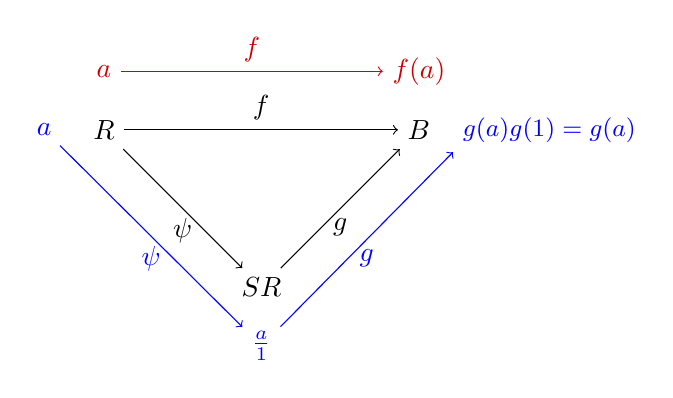
\begin{tikzpicture}
			\node (R) at (0,0) {$R$};
			\node (SR) at (2,-2) {$\inv{S}R$};
			\node (B) at (4, 0) {$B$};

			\draw[->] (R) -- node[midway, below] {$\psi$} (SR);
			\draw[->] (SR) -- node[midway, below] {$g$} (B);
			\draw[->] (R) -- node[midway, above] {$f$} (B);

			\node[blue, xshift = -0.5cm] (A) at (R.west) {$a$};
			\node[blue, xshift = 0.7cm, anchor = west] (AB) at (B.west) {\small $g(a)·\inv{g(1)} = g(a)$};
			\node[blue, yshift=-0.5cm] (A1) at (SR.south) {$\frac{a}{1}$};

			\draw[->, blue] (A) -- node[midway, below] {$\psi$} (A1);
			\draw[->, blue] (A1) -- node[midway, below] {$g$} (AB.south west);

			\node[red!80!black, yshift = 0.5cm] (FA) at (R.north) {$a$};
			\node[red!80!black, yshift = 0.5cm] (FB) at (B.north) {$f(a)$};

			\draw[->, red!80!black] (FA) -- node[midway, above] {$f$} (FB);
			\end{tikzpicture}
		\end{center}

		Por tanto, como el diagrama conmuta $g(a)=f(a)$, lo que nos deja fijo el comportamiento de $g$ en los elementos de la forma $\frac{a}{1}$ con $a ∈ R$. Nos falta saber qué ocurre con los que no son de esa forma, y saber si ahí también tenemos una única posibilidad de tomar $g$.

		Para eso, sólo tenemos que ver qué ocurre a los elementos de la forma $\frac{1}{s}$. Operando: \[ g\left(\frac{1}{s}\right)=g(1)g(s^{-1})=g(s^{-1})=g(s)^{-1}=f(s)^{-1} \], ya que por hipótesis $f(s)$ con $s ∈ S$ son elementos invertibles. Por lo tanto, $g$ es única y depende solamente de la elección de la $f$ de partida.

		\proofpart{Existencia}

		Ahora vamos a probar que existe esa $g$. Si $g$ existiese tendríamos $g\left( \frac{r}{s}\right)=f(r)f(s)^{-1}$. Tenemos que ver que $g$ está bien definida (que dos elementos iguales no tengan imágenes distintas), es decir, que la expresión anterior no dependa del representante escogido.

		Supongamos que $\frac{r}{s} \equiv \frac{r'}{s'}$, hay que ver que $g\left(\frac{r}{s}\right)=g\left(\frac{r'}{s'}\right)$. Es decir, que $f(r)f(s)^{-1}=f(r')f(s')^{-1}$.

		Como  $\frac{r}{s} \equiv \frac{r'}{s'}$, entonces existe $s'' \in S$ tal que $s''(rs'-sr')=0$ en $R$. Aplicando f nos queda:
		$$f(s''(rs'-sr'))=f(s'')\left( f(r)f(s')-f(s)f(r') \right)=0$$

		Por hipótesis $f(s'')$ es invertible, por tanto, es una unidad en $B$, entonces no es un divisor de 0 y por tanto:
		$$f(r)f(s')-f(s)f(r')=0 \implies f(r)f(s')=f(s)f(r')$$

		Y multiplicando por la inversa de $f(s')$ y de $f(s)$, nos queda $f(r)f(s)^{-1}=f(r')f(s')^{-1}$.
	\end{proof}

	\begin{example}
		Sea $\rac[x]$, cogemos como parte multiplicativa $S=\{x^n\}$.

		Los elementos de $S^{-1}\rac[x]$ serán de la forma $\frac{p(x)}{x^m}$.

		\notacion $S^{-1}\rac[x]=\rac[x]_{\{x\}}$

		Defino el siguiente diagrama:

		\begin{center}
		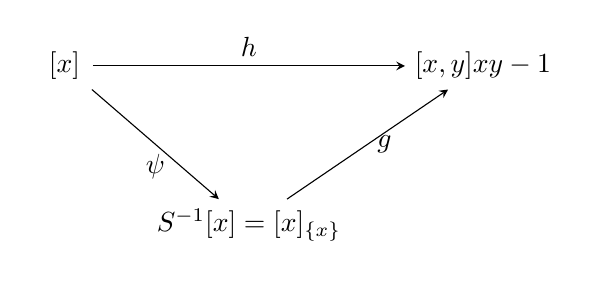
\begin{tikzpicture}
		\matrix (m) [matrix of math nodes,row sep=4em,column sep=2em,minimum width=2em]
		{
			\rac[x] &  & \quot{\rac[x,y]}{\gen{xy-1}} \\
			& S^{-1}\rac[x]=\rac[x]_{\{x\}}  &  \\};
		\path[-stealth]
		(m-1-1) edge node [above] {$h$} (m-1-3)
		(m-1-1) edge node [below] {$\psi$} (m-2-2)
		(m-2-2) edge node [right] {$g$} (m-1-3);
		\end{tikzpicture}
		\end{center}

		Vemos que $\cls{x}\cls{y}=\cls{1} \implies x^{-1}=y \implies (x^m)^{-1}=y^m$. Con esto hemos visto que $h(s)$ es invertible $\forall s \in S$.

		La propiedad universal me dice que tengo un único homomorfismo $g: \rac[x]_{\{x\}}\longmapsto \quot{\rac[x,y]}{\gen{xy-1}}$

	\end{example}

	\begin{theorem} \label{thm:PropsLocalizacion}
		Sea $S \subset R$ una parte multiplicativa. El homomorfismo de paso al localizado $\psi:R \longmapsto S^{-1}R$ tiene las siguientes propiedades:
		\begin{enumerate}
			\item Si $s\in S$, $\psi(s)$ es invertible en $S^{-1}R$.
			\item $\psi(a)=0 \Leftrightarrow \exists s \in S$ tal que $s\cdot a=0$.
			\item Cada elemento de $S^{-1}R$ es de la forma $\psi(r)\psi(s)^{-1}$
		\end{enumerate}

		Estas propiedades determinan completamente a $S^{-1}R$ de tal modo que si $f:R \longmapsto B$ es un homomorfismo de anillos tal que se cumplen $1), 2), 3)$ (cambiando $S^{-1}R$ por $B$) entonces $S^{-1}R \simeq B$.
	\end{theorem}

	\begin{proof}
		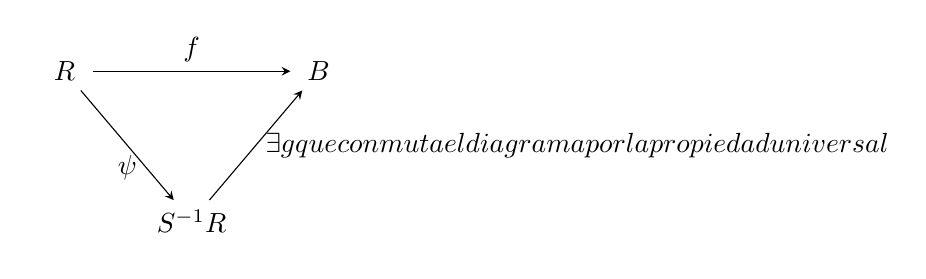
\begin{tikzpicture}
		\matrix (m) [matrix of math nodes,row sep=4em,column sep=2em,minimum width=2em]
		{
			R &  &  B\\
			& S^{-1}R &  \\};
		\path[-stealth]
		(m-1-1) edge node [above] {$f$} (m-1-3)
		(m-1-1) edge node [below] {$\psi$} (m-2-2)
		(m-2-2) edge node [right] {$\exists g \text{ que conmuta el diagrama por la propiedad universal}$} (m-1-3);
		\end{tikzpicture}

		Veamos que ese $g$ es un isomorfismo:
		\begin{itemize}
			\item \textbf{g es sobreyectiva:} Si, por $3)$, todo elemento $a \in B$ es de la forma $f(r)f(s)^{-1}$. Tenemos que ver que para todo elemento de $B$ hay una preimagen en $S^{-1}R$ Basta observar que $g\left( \frac{r}{s} \right) f(r)f(s)^{-1}$.
			\item \textbf{g es inyectiva:} Si porque:
			$$\ker(g) = \{ \frac{r}{s}: g(r)g(s)^{-1}=0_B \} = \{ \frac{r}{s}: f(r)f(s)^{-1}=0_B \} = $$

			Y como $f(s)^{-1}$ es invertible, no es divisor de 0 y por tanto:

			$$ = \{ \frac{r}{s}: f(r)=0_B \} \implies r \in \ker(f) \implies r \in \ker(\psi)\textcolor{red}{???}$$
		\end{itemize}
	\end{proof}

\section{Ideales y localización}

\nota Esto es elemental, pero yo a veces lo dudaba. Sea cualquier función $f: A \longmapsto B$:
\begin{itemize}
	\item Sea un conjunto $M \subset B$, entonces $f(f^{-1}(M)) \subset B$.

	Intuitivamente, al hacer $f^{-1}(M)$ te quedas con los $x \in A$ tal que $f(x) \in M$, pero no todos los $m \in M$ tienen porque tener una preimagen $x \in A$..., por tanto es ahi donde empequeñece el conjunto. Si $f$ es sobreyectiva entonces $f(f^{-1}(M))= B$.
	\item Sea un conjunto $N \subset A$, entonces $f^{-1}(f(N)) \supset A$.

	Intuitivamente, al hacer $f(N)$ te quedas con los $y \in B$ tal que $f(x)=y$, con $x\in N$, pero puede que haya valores de $y$ que sean la imagen de dos valores distintos de $x$, y que alguno de ellos no pertenezca a $N$, es al hacer la preimagen de esos $y$ cuando podemos agrandar el conjunto. Si $f$ es inyectiva entonces $f^{-1}(f(N)) =  A$.
\end{itemize}

Vamos con lo importante, enunciaremos y demostraremos 4 proposiciones sobre ideales y localización. A lo largo de esta sección, consideraremos $\appl{\psi}{R}{S^{-1}R}$ nuestra aplicación de paso al localizado.

En general, si cogemos un ideal $J \subset S^{-1}R$, entonces $\psi^{-1}(J)$ es ideal en $R$. Pero si volvemos a tomar la imagen por ψ no tiene por qué ser un ideal. En secciones anteriores habríamos que podemos considerar el ideal extendido que sí está contenido en $J$: $\psi(\psi^{-1}(J))^e \subset J$. En el caso particular del paso al localizado, tendremos una igualdad.

\begin{prop}
	Sea $\psi:R \longmapsto S^{-1}R$ el homomorfismo de paso al localizado, y sea el ideal $J \subset S^{-1}R$.  Entonces $\psi(\psi^{-1}(J))^e = J$.
\end{prop}

\begin{proof}
	Ya tenemos $\psi(\psi^{-1}(J))^e \subset J$. Por tanto probamos $\psi(\psi^{-1}(J))^e \supset J$:

	Consideramos un elemento $\frac{b}{s} \in J$. Por ser $J$ ideal, tenemos que $\frac{b}{s} \frac{s}{1} = \frac{b}{1} ∈ J$, y su imagen inversa será $b ∈ \inv{ψ}(J)$.

	Ahora simplemente hacemos el camino de vuelta: $ψ(b) = \frac{b}{1} ∈ ψ(\inv{ψ}(J)) ⊂ \psi(\psi^{-1}(J))^e$. Como este último es un ideal, multiplicamos de nuevo $\frac{b}{1}$ por $\frac{1}{s}$ para tener por absorción que $\frac{b}{s} ∈ \psi(\psi^{-1}(J))^e$.
\end{proof}


\obs Todo ideal de $S^{-1}R$ es el extendido de algún ideal de $R$.

Si partimos de un ideal en $R$, también podemos tener un resultado para $\psi^{-1}(\psi(I)^e) $ que contendrá a $I$ (y quizás sea igual a él). Ahora bien, no será tan fácil como el anterior. Vamos a ver primero algunos ejemplos.

\begin{example}
	\begin{itemize}
		\item Sea $\psi: \ent \longmapsto \rac$. $\rac$ es localizado de $\ent$, haciendo invertible $S=\rac \setminus\gen{0}$. Nos queda $\rac=S^{-1}\ent$.

		Si cojo $I=2\ent \implies \psi(I)^e=\rac \implies \psi^{-1}(\psi(I)^e)= \ent$

		\item Sea $S=\{ 2^n \}$, $\psi: \ent \longmapsto S^{-1}\ent$

		Sea $I=6\ent\implies 6\frac{1}{2}=3 \in \psi(I)^e$... ejemplo sin terminar...
	\end{itemize}
\end{example}

\begin{prop}
	$$\psi^{-1}(\psi(I)^e)=\bigcup_{s\in S}(I:S)$$

	Con $(I:S)=\{ r \in R: r\cdot S \in I \}$.
\end{prop}

\begin{proof}
	\begin{itemize}
		\item $\supset)$ Sea $r \in \bigcup_{s\in S}(I:S) \implies \exists s' \in S$ tal que $r \in (I:s')\implies r\cdot s' \in I \implies \frac{r \cdot s'}{1} \in \psi(I) \textcolor{red}{\implies} \frac{r}{1} \in \psi(I)^e \implies r \in \psi^{-1}(\psi(I)^e)$
		\item $\subset$ Sea $r \in \psi^{-1}(\psi(I)^e)\implies \frac{r}{1}\in \psi(I)^e \implies \frac{r}{1}=\frac{r_1}{s_1}a_1+...+\frac{r_t}{s_t}a_t$ con $a_1,...,a_t \in I \implies s''\frac{r}{a}\in I$ con $s''=s_1...s_t \implies r \in (I:s'')$
	\end{itemize}
\end{proof}

\begin{prop} $\psi^{-1}(\psi(I)^e)=R \Leftrightarrow I \cap S \neq \emptyset$.
\end{prop}

\begin{prop}
	Sea $\pideal \subset R$ un ideal primo, entonces:
	\begin{itemize}
		\item Si $\pideal \cap S \neq \emptyset \implies \psi(\pideal)^e=S^{-1}R$.
		\item Si $\pideal \cap S = \emptyset \implies \psi(\pideal)^e$ es un ideal primo en $S^{-1}R$.
	\end{itemize}
\end{prop}

\begin{proof}
	Vamos a probar que $\psi(\pideal)^e$ es primo.

	Tenemos que $\psi(\pideal)^e\neq \gen{1}$ porque $\pideal \cap S= \emptyset$

	Sean $\frac{r}{s},\frac{r'}{s'} \in S^{-1}R$ tal que $\frac{r}{s}\cdot\frac{r'}{s'} \in \psi(\pideal)^e$.

	Entonces $\frac{r}{s}$ o $\frac{r'}{s'} \in \psi(\pideal)^e \implies \frac{r}{s}\cdot\frac{r'}{s'}=\frac{r_1}{s_1}a_1+...+\frac{r_t}{s_t}a_t$ con $a_1,...,a_t \in \pideal$ y $s_1,...,s_t \in S$.

	Sea $s''=s\cdot s' \cdot s_1 \cdot...\cdot s_t \in S$. Definimos: $\cls{s}=\frac{s''}{s\cdot s'} \in S \subset R$. Entonces:
	$$ \underbrace{\frac{s''}{s\cdot s'}}_{\in S \subset R}\cdot r \cdot r'=\underbrace{s''\frac{r_1}{s_1}a_1+...+s''\frac{r_t}{s_t}a_t}_{\text{comb lineal sobre R de elementos de }\pideal} $$

	Por tanto $(\cls{s})\cdot(r \cdot r') \in \pideal$ que es primo $\implies \underbrace{\cls{s}\in p}_{\textbf{No porque}\pideal \cap S = \emptyset}$ o $r\cdot r' \in \pideal \implies r \cdot r' \in \pideal \implies r$ o $r' \in \pideal$.

	Si $r \in \pideal \implies \frac{r}{1} \in \psi(\pideal)$ y $\frac{r}{s} \in \psi(\pideal)^e$. Si no, de igual modo se prueba que entonces $\frac{r'}{s'}\in \psi(\pideal)^e$.
\end{proof}

Las conclusiones de estas tres proposiciones son \textbf{IMPORTANTES}:
\begin{enumerate}
	\item Todo ideal de $S^{-1}R$ es el extendido de algún ideal de $R$.
	\item Hay una correspondencia biyectiva entre ideales primos $p \subset R$, $p \cap S = \emptyset$ y los ideales primos de $S^{-1}R$.
\end{enumerate}

\notacion
\begin{itemize}
	\item Sea $S \subset R$, $S=\{ a^n \}, a \in R$. Entonces $S^{-1}R=R_a=R_{\{a\}}$. A esto se le llama ``R localizado en a'' o \concept{Localización\IS en un elemento}.
	\item Sea $S=R \setminus \pideal$ con $\pideal \subset R$ ideal primo en $R$. Entonces $S^{-1}R=R_\pideal$. A esto se le llama ``R localizado en el ideal primo $\pideal$'' o \concept{Localización\IS en un ideal primo}, y además $R_\pideal$ es un anillo local.
\end{itemize}


Sea $R=\ent$, no confundir: $\ent_{\{3\}}$, con $\ent_{\gen{3}}$ con $\ent_3$, son todos distintos. Observar que con $R=\ent$ es diferente $R_a$ y $R_{\{a\}}$.
\begin{itemize}
	\item $\ent_{\{3\}}$ es un subanillo de los racionales en el que sólo nos quedamos con aquellos números racionales que admiten una escritura cuyo denominador es una potencia de 3.
	\item $\ent_{\gen{3}}$ es un subanillo de los racionales en el que sólo nos quedamos con aquellos números racionales que admiten una escritura cuyo denominador no es un múltiplo de 3.
	\item $\ent_3=\{ \cls{0},\cls{1},\cls{2} \}$ que no tiene nada que ver con todo esto.
\end{itemize}

\section{Anillos noetherianos}
\begin{defn}[Anillo\IS noetheriano] \label{def:AnilloNoetheriano}
	Se dice que $R$ es un anillo noetheriano si todo ideal $I \subset R$ es finitamente generado (como $R$-módulo). (ver \nref{def:rmodulo_fg})

	%Es decir, que para todo ideal en R  puedo encontrar un número finito de elementos dentro del ideal, de modo tal que cualquier otro elemento que viva en el ideal se puede escribir como combinación lineal de ellos.
\end{defn}

\begin{example}
	\begin{itemize}
	\item $\ent$ es noetheriano, porque es dominio de ideales principales, es decir, todos sus ideales son principales (ver \nlref{def:ideal_principal}).
	\item $K$ cuerpo es noetheriano, porque en un cuerpo solo hay dos ideales, $\{0\}$ y $K$, ambos finitamente generados.
	\item $K[x]$ es noetheriano, porque es dominio de ideales principales.
	\item $K[x_1,...,x_n]$, $\rac[x,y]$ y $\ent[x]$ son noetherianos, pero hay que demostrarlo.
	\item $K[x_1,...,x_n,...]$, con número infinito de variables no es noetheriano.

	Cogemos $I \subset K$, $I= \{ p(\cls{x}): \text{término constante igual a 0} \}$.

	\notacion $\cls{x}=\{x_1,x_2,...,x_n,...\}$
	\nota En $I$ no existe el polinomio $p(\cls{x})=x_1+x_2+...+x_n+...$ ya que no se pueden sumar un número infinito de sumandos. Las combinaciones lineales finitas sí están.

	Entonces tenemos que $I$ es un ideal (cumple las tres condiciones de los ideales), y que $p(\cls{x})=x_i \in I$ $ \forall i$. Pero $I$ no es finitamente generado.
	\begin{proof}
		Supongamos que $\exists p_1,...,p_s \in K[x_1,...,x_n,...]$ tal que $I=\gen{p_1,...,p_s}$, tal que $p_1,...,p_s$ solo dependen de un número finito de variables.

		Supongamos sin pérdida de generalidad que sólo dependen de $x_1,...,x_n$.

		Entonces es imposible escribir $x_{n+1}$ como combinación de los $p_i$. $x_{n+1}\neq q_1p_1+...+q_sp_s$, como mucho obtenemos productos $x_ix_{n+1}$, pero nunca $x_{n+1}$ solo.
	\end{proof}
	\end{itemize}
\end{example}

\begin{prop}\label{prop:caracterizacion_noetheriano}
	Son equivalentes:
	\begin{enumerate}
		\item $R$ es noetheriano.
		\item Toda cadena creciente de ideales en $R$, $\{I_i\}_{i \in \nat}$ estabiliza para un $n$ suficientemente grande: $I_1 \subseteq I_2 \subseteq ... \subseteq I_n = I_{n+1}$.
		\item Todo conjunto no vacío de ideales en $R$ tiene un elemento maximal (No tiene por qué ser un ideal maximal).
	\end{enumerate}
\end{prop}

\begin{proof}

		\proofpart{$1) \implies 2)$}

		Sea $R$ un anillo noetheriano y sea $\{I_i\}_{i \in \nat}$ una cadena creciente de ideales en $R$. Queremos probar que la cadena estabiliza para algún $N$ suficientemente grande.

		Sea $J= \bigcup_{i \in \nat} I_i$. Entonces $J$  es un ideal en $R$. En general la union de ideales no tiene porque ser un ideal, pero en el caso de ser una cadena creciente sí lo es (mirar demostración del teorema \ref{thm:IdealContenidoMaximal}). Como $R$ es noetheriano, $J$ es finitamente generado, por tanto existen $a_1,...,a_s \in J$ tal que $J=\gen{a_1,...,a_s}$.

		Además tenemos que $I_1 \subseteq I_2 \subseteq ... \subseteq I_N \subseteq ...$, por tanto, $\exists k$ tal que  $a_1,...,a_s \in I_k = J = \gen{a_1,...,a_s}$

		\proofpart{$2) \implies 3)$}

		Sea $\Sigma$ un conjunto no vacío de ideales en $R$, queremos probar que tiene un elemento maximal.

		Supongamos que en $\Sigma$ hay una cadena creciente de ideales $\{I_i\}$. Por la hipótesis en $2)$, la cadena estabiliza, luego tiene un elemento maximal.

		Si esa cadena no existe, se construye. Tenemos un conjunto de ideales $\set{I_i}$, así que construimos la cadena $I_1 ⊆ I_1 ∪ I_2 ⊆ I_1 ∪ I_2 ∪ I_3 ⊆ \dotsb$ y aplicamos lo de antes\footnoteby{Guille}{No tengo claro qué hacer si el conjunto de ideales es no numerable. Ahora bien, parece que ese no es un caso que estemos considerando en ningún momento.}.

		\proofpart{$3) \implies 1)$}

		Sabemos que todo conjunto no vacío de ideales en $R$ tiene un elemento maximal, y queremos probar que $R$ es noetheriano.

		Sea $I \subset R$, supongamos que $I\neq \{0\}$ y que $I$ no es finitamente generado.
		\begin{itemize}
			\item Sea $a_1 \in I, a_1 \neq 0$.
			\item Sea $a_2 \in I\setminus \gen{a_1}$. Puedo encontrar ese $a_2$ porque si no lo encontrara querría decir que $I$ sería finitamente generado.
			\item Sea $a_3 \in I\setminus \gen{a_1,a_2}$.
			\item Sea $a_n \in I\setminus \gen{a_1,...,a_n}$.
		\end{itemize}
		Considero $\gen{a_1}\subsetneq \gen{a1,a2} \subsetneq \gen{a_1,a_2,a_3} \subsetneq...$. Esta cadena creciente de ideales nunca estabiliza. Lo cual es contradictorio porque entonces podría haber definido $\Sigma=\{ \gen{a_1}, \gen{a_1},\gen{a_1,a_2},...,\gen{a_1,a_2,...,a_n},.... \} \neq \emptyset$ y no tiene elemento maximal.
\end{proof}

\begin{theorem}[Teorema\IS de la base de Hilbert]\label{thm:tma_base_hilbert}
	Sea $R$ un anillo noetheriano. Entonces $R[x]$ es un anillo noetheriano.
\end{theorem}

\begin{proof}
	Sea $I \subset R[x]$, queremos probar que $I$ es finitamente generado.
	\nota El coeficiente director de un polinomio es el coeficiente que acompaña al término de mayor grado.
	\nota El grado es un numero $a \in \nat$, y los $\nat$ son ordenables, por tanto, si hablamos de grado mínimo, que no nos extrañe, es lo que todos pensamos: el grado menor.

	Vamos a suponer que $I$ no es finitamente generado, podemos suponer que $I\neq \{0\}$, así:
	\begin{itemize}
		\item Sea $f_1(x) \in I$ con grado mínimo, sea $a_1$ el coeficiente director de $f_1(x)$.
		\item Sea $f_2(x) \in I\setminus \gen{f_1(x)}$ con grado mínimo, puedo cogerlo ya que hemos supuesto que $I$ no es finitamente generado, sea $a_2$ el coeficiente director de $f_2(x)$.
		\item Sea $f_{k+1}(x) \in I\setminus \gen{f_1(x),...,f_k(x)}$ con grado mínimo, sea $a_{k+1}$ el coeficiente director de $f_k(x)$.
	\end{itemize}

	Entonces, con los coeficientes directores puedo montar la siguiente cadena: $\gen{a_1} \subseteq \gen{a_1,a_2} \subseteq ... \subseteq \gen{a_1,...,a_k,a_{k+1}}$, que es una cadena creciente de ideales de $R$, además sabemos por hipótesis que $R$ es noetheriano, por tanto esa cadena se debe estabilizar.

	Pero hemos supuesto que $I$ no es finitamente generado, y afirmamos que si eso ocurre, la cadena anterior no puede estabilizar, vamos a probar eso:

	Supongamos que estabiliza $\implies$ para algún $k$ se cumple que $\gen{a_1,...,a_k}=\gen{a_1,...,a_k,a_{k+1}} \implies \exists b_1,...,b_k \in R$ tal que: $a_{k+1}=b_1a_1+...+b_ka_k$. Donde $a_{k+1}$ es el coeficiente director de $f_{k+1}(x)$. Defino:

	\textcolor{red}{Revisar el final de esta demostracion}

	$$ g=f_{k+1}(x)-\sum_{i=1}^{k}b_ix^{\deg(f_{k+1}(x))-\deg(f_i(x))} f_i(x) \in I\setminus \gen{f_1,...,f_k} $$

	%Como las $f_i$ tiene grado igual o mayor, estoy haciendo es obtener justamente el a_{k+1} con signo negativo.

	Tenemos que $\deg(g) < \deg(f_{k+1}(x))$. Lo cual es contradictorio porque $g \in I \setminus \gen{f_1,...,f_k}$ y tiene grado < $\deg(f_{k+1})$.

\end{proof}

\begin{example}
	\begin{itemize}
	\item $\ent[x_1,...,x_n]$ es noetheriano. No hay más que coger $\ent$, que sabemos que es noetheriano, y 'aplicar' el teorema anterior n veces.
	\item $\K[x_1,...,x_n]$ es noetheriano por el mismo motivo.
	\item Si $R$ es noetheriano $\implies$ $R[x_1,...,x_n]$ es noetheriano.
	\end{itemize}
\end{example}

\subsection{Anillos noetherianos y paso al cociente}

\begin{prop} \label{prop:NoetherianoCociente}
	Sea $R$ un anillo noetheriano y sea $I \subset R$ un ideal $\implies$ $\quot{R}{I}$ también es noetheriano.
\end{prop}
\begin{proof}
	Sea $\pi: R \longmapsto \quot{R}{I}$, tenemos que probar que $J \subset \quot{R}{I}$ es finitamente generado.

	Cogemos $L \subset R$ ideal de $R$ tal que $I \subset L$ y tal que $\pi(L)=J$ ($L$ es posible de encontrar, ver \ref{relacionRconRI}, relación entre los ideales de $R$ y $\quot{R}{I}$, apartado 2). Como $R$ es noetheriano, $L$ es finitamente generado, es decir, $\exists a_1,...,a_s \in L$ tal que $L=\gen{a_1,...,a_s} \implies J=\gen{\pi(a_1),...,\pi(a_s)}$.

	También se puede probar utilizando la segunda caracterización de los anillos noetherianos (ver proposición \ref{prop:caracterizacion_noetheriano}). Cualquier cadena creciente de ideales en $R$ estabiliza, si me fijo en una cadena creciente de ideales en $\quot{R}{I}$, viene de una cadena creciente de ideales en $R$, por la correspondencia biyectiva.
\end{proof}

Una consecuencia de lo anterior es:

\obs Sea $R$ un anillo noetheriano y sea $T$ una $R$-álgebra de tipo finito (ver definición de $R$-álgebra finitamente generada: \ref{def:ralgebra_fg}). Entonces $T=R[b_1,...,b_n]$ para ciertos $b_1,...,b_n \in T$. De hecho $T=R[b_1,...,b_n]$ es también noetheriano.

\begin{proof}
	Sea $R$ un anillo noetheriano, le añadimos n variables (sigue siendo noetheriano por el teorema de Hilbert \ref{thm:tma_base_hilbert}) y definimos el siguiente homomorfismo de $R$-álgebras:

	\begin{align*}
		\psi: R[x_1,...,x_n] & \longmapsto  T=R[b_1,...,b_n]\\
		r \in R & \longmapsto r \\
		x_i & \longmapsto b_i \\
	\end{align*}

	Entonces $\psi$ es un homomorfismo de $R$-álgebras y es sobreyectivo por cómo lo hemos construido. Ahora aplicamos el primer teorema de isomorfía:
	$$ \quot{R[x_1,...,x_n]}{\ker(\psi)} \simeq \img(\psi)=T=R[b_1,...,b_n]$$

	Por tanto tenemos:
	 $$\quot{\text{anillo noetheriano}}{\text{ideal}}$$

	Y como hemos visto antes, eso es noetheriano. Por tanto: $T=R[b_1,...,b_n]$ es noetheriano.
\end{proof}

\begin{example}
	\begin{itemize}
		\item $\rac[\sqrt{2},x, \pi]$ es una $\rac$-álgebra.
		\item $\real$ es una $\rac$-álgebra pero no de tipo finito.
	\end{itemize}
\end{example}

\subsection{Anillos noetherianos y localización}

\begin{prop} \label{prop:NoetherianoLocalizacion}
	Sea R un anillo noetheriano y sea $S\subset R$ una parte multiplicativa. Construimos como otras veces el siguiente homomorfismo:
	$$\psi: R \longmapsto S^{-1}R$$

	Entonces $S^{-1}R$ es noetheriano.
\end{prop}
\begin{proof}
	Para ello tenemos que probar que sea $J \subset S^{-1}R$ un ideal, este es finitamente generado.

	Lo cual es cierto ya que $J$ es el extendido de algún ideal de $R$ y hemos probado que $\psi(\psi^{-1}(J))^e=J$. Por tanto $J$ es el extendido de $\psi^{-1}(J)\subset R \implies J$ es finitamente generado. \textcolor{red}{Revisar cuando repase lo que dimos esos días...} %min 19
\end{proof}



% -*- root: ../AlgebraConmutativa.tex -*-

% Clase 7/3/2016
Vamos a ver algunas propiedades de estas variedades generadas por ideales. Por ejemplo, si tomamos dos ideales $J, I ⊂ K[x_1, \dotsc, x_n]$, si $J ⊂ I$ entonces $\V(J) ⊃ \V(I)$.

Los radicales también nos darán resultados interesantes. A priori, un radical nos debería dar una variedad más pequeña al ser un ideal más grande. La cuestión es que lo que nos dará en realidad será la misma variedad.

\begin{prop} Sea $I ⊂ K[x_1, \dotsc, x_n]$ un ideal, y consideramos su radical $\sqrt{I}$. Entonces $\V(I) = \V(\sqrt{I})$.
\end{prop}

\begin{proof}

\proofpart{$⊃$}

Como $I ⊂ \sqrt{I}$, es obvio que $\V(I) ⊃ \V(\sqrt{I})$.

\proofpart{$⊂$}

Lo primero que tenemos que hacer es tener cuidado cuando el ideal es el vacío. Ahora bien, si $\V(I) = ∅$, entonces $\V(\sqrt{I}) = ∅$ igualmente, ya que hemos demostrado antes que $\V(\sqrt{I}) ⊂ \V(I)$.

Podemos suponer entonces que $\V(I) ≠ ∅$. Sea $(a_1, \dotsc, a_n) ∈ \V(I)$ o, en otras palabras, que $∀p(x_1, \dotsc, x_n) ∈ I$ se tiene que $p(a_1, \dotsc, a_n) = 0$.

Queremos demostrar que $(a_1, \dotsc, a_n) ∈ \V(\sqrt{I})$ y por lo tanto que $∀q(x_1, \dotsc, x_n) ∈ \sqrt{I}$ tengamos que $q(a_1, \dotsc, a_n) = 0$. Ahora bien, por ser $q$ elemento del radical, elevado a una potencia $m > 0$ nos dará cero, luego en particular $q(a_1, \dotsc, a_n)^m = 0$. Pero $q(a_1, \dotsc, a_n) ∈ K$ que es un cuerpo y dominio de integridad, así que si elevado a una potencia nos da $0$ tiene que ser él mismo cero, y por lo tanto $(a_1, \dotsc, a_n) ∈ \V(\sqrt{I})$.
\end{proof}

\subsection{La operación $\I(S)$}

Vamos a tomar un subconjunto $S ⊂ \A_K^n$. Nos fijaremos en todos los polinomios en $n$ variables que se anulan en $S$. Es decir, \[ \I(S) = \set{p(x_1, \dotsc, x_n) ∈ K[x_1, \dotsc, x_n] \tq ∀(a_1, \dotsc, a_n) ∈ S \; p(a_1, \dotsc, a_n) = 0} \]

No es difícil ver que $\I(S)$ es un ideal: no es vacío ($0 ∈ \I(S)$), está cerrado con la suma y la propiedad de absorción también se cumple trivialmente.

\begin{wrapfigure}{R}{0.4\textwidth}
\centering
\begin{tikzpicture}
\draw[->] (-0.5, 0) -- (3,0);
\draw[->] (0, -0.5) -- (0,2);

\draw[|-|, very thick, blue] (0,0) node[anchor = north west, yshift = -0.05cm, xshift = -0.05cm] {$0$} -- (1,0) node[below, yshift = -0.05cm] {$1$};
\end{tikzpicture}
\caption{El intervalo $[0,1]$ no es una variedad algebraica.}
\label{fig:Interv01}
\end{wrapfigure}

Por ejemplo, podemos buscar todos los polinomios que se anulan en el intervalo $S= [0,1]$. Está claro que $\gen{y} = \I(S)$, pero no vamos a poder encontrar un polinomio que se anule sólo en $S$. La razón es que $S = [0,1]$ no es una variedad algebraica. Esto nos va a dar un lema interesante.

\begin{lemma} Sea $S ⊂ \A_K^n$ un subconjunto del espacio afín. Entonces $\V(\I(S)) ⊃ S$, y la igualdad $\V(\I(S)) = S$ se da si y sólo si $S$ es una variedad algebraica afín.
\end{lemma}

\begin{proof} Por definición, siempre tenemos que $S ⊂ \V(\I(S))$. Supongamos que $S = \V(\I(S))$. Es claro que $S$ es una variedad algebraica afín, porque la igualdad indica que $S$ es el conjunto de ceros del ideal $\I(S)$.

Vamos a ir con la demostración al otro lado. Supongamos que $S$ es una variedad algebraica afín, y queremos demostrar que $S = \V(\I(S))$.

Como $S$ es una v.a.a., entonces $∃ J ⊂ K[x_1, \dotsc, x_n]$ tal que $S = \V(J)$, luego $J ⊂ \I(S)$. Entonces podemos hacer una cadena \[ S = \V(J) ⊃ \V(\I(S)) ⊃ S \], por lo que todas las inclusiones tienen que ser igualdades.
\end{proof}

Este lema lo podemos relacionar con la topología de Zariski que veíamos antes, que nos decía que los cerrados eran las variedades algebraicas.

\begin{corol} Sea $S ⊂ \A_K^n$. Entonces la \concept{Clausura\IS de Zariski} de $S$ es $\adh{S} = \V(\I(S))$, y entonces $\adh{S}$ es la variedad algebraica más pequeña que contiene a $S$.
\end{corol}

\begin{proof}
Sabemos que $S ⊂ \V(\I(S))$, donde $\V(\I(S))$ es una variedad algebraica afín. Tenemos que probar que además es la variedad más pequeña que contiene a $S$.

Hacemos la demostración por reducción al absurdo, suponiendo que existe una variedad algebraica afín $X ⊃ S$ y además $X \subsetneq \V(\I(S))$. Ahora bien, es obvio que $\I(S) ⊃ \I(X) ⊃ \I(\V(\I(S)))$. Podemos volver a tomar la variedad y entonces \[ \V(\I(S)) ⊂ \underbracket{\V(\I(X))}_{ = X} ⊂ \underbracket{\V(\I(\V(\I(S))))}_{= \V(\I(S)))} \], luego $X = \V(\I(S))$, contradicción.
\end{proof}

Dos observaciones:

\begin{prop}
Dado $S ⊂ \A_K^n$, el ideal $\I(S)$ es un ideal radical.
\end{prop}

\begin{proof} Ejercicio para el lector.
\end{proof}

\begin{prop} Sea $X ⊂ \afesp$ una variedad algebraica afín. Entonces existe $J ⊂ K[x_1, \dotsc, x_n]$ tal que $\V(J) = X$.
\end{prop}

El ideal $J$ no es el único que determina a $X$. Sin embargo, el ideal $\I(X)$ es el ideal más grande de $K[x_1, \dotsc, x_n]$ cuyos ceros son $X$, esto es, es el ideal más grande tal que $X = \V(\I(X))$.

Esto nos permite asociar un ideal radical a $X$ sin ninguna ambigüedad. Diremos entonces que $I(X)$ es el ideal que determina a $X$.

\chapter{Teorema de los ceros de Hilbert}

Hemos jugado en $\Akn$ y en $\K[x_1,...,x_n]$. Y sabemos movernos de un sitio a otro:

\begin{align*}
	\Akn & \longmapsto  \K[x_1,...,x_N] \\
	X & \longmapsto  \I(X) \\
	\V(J) & \leftarrow  J \\
\end{align*}

\begin{itemize}
	\item Si cojo $X\in \Akn$ v.a.a., puedo ir a $\I(X) \in \K[x_1,...,x_n]$ y volver a $\V(\I(X)) \in \Akn$ que es igual a $X$ por ser una v.a.a..

	Tendría el siguiente diagramilla:

	\item Sin embargo, si cojo $J$ ideal radical en $\K[x_1,...,x_n]$, puedo ir a $\V(J)$ en $\Akn$, y volver a $\I(\V(J)) \supseteq J$. Pero puede pasar que la inclusión sea estricta:
	\begin{example}
		\textcolor{red}{Julian majo pon esto mas bonito}
		\begin{enumerate}
			\item Ejemplo de inclusión estricta:
			\begin{align*}
				\A^1_{\real} & \longmapsto  \real[x] \\
				\V(\gen{x^2+1}) & \leftarrow  \gen{x^2+1} \\
				\shortparallel & \\
				\emptyset & \longmapsto  \I(\{ \emptyset \})=\real[x] \\
			\end{align*}
			\item Otro ejemplo de inclusión estricta:

			Cogemos en $\real[x,y]$ e ideal  radical $\gen{(x-1)^2+(y-2)^2}$, que es primo (y por tanto radical) porque $p(x,y)=(x-1)^2+(y-2)^2$ es irreducible en $\real[x,y]$.

			Esto es así porque $\real[x,y] \subset \cplex[x,y]$  que es un dominio de factorización única.

			Y en $\cplex[x,y]$ tenemos que $p(x,y)=(x-1)^2+(y-2)^2=((x-1)+i(y-2))((x-1)-i(y-2))$. Por tanto no se puede factorizar de otra forma.

			\begin{align*}
				\A^2_{\real} & \longmapsto  \real[x,y] \\
				\V(J) & \leftarrow  \gen{(x-1)^2+(y-2)^2}=J \\
				\shortparallel & \\
				X=\{1,2\} & \longmapsto  \I(X)=\gen{x-1,y-2}\\
			\end{align*}

			Y obviamente $\gen{(x-1)^2+(y-2)^2} \subsetneqq \gen{x-1,y-2}$
		\end{enumerate}
	\end{example}
\end{itemize}

\textbf{Conclusión:} No hay un diccionario entre v.a.a. en $\Akn$ e ideales radicales en $\K[x_1,...,x_n]$.

\begin{theorem}[Teorema de los ceros de Hilbert]\label{teor:tma_0_hilbert}
	Si $\K$ es algebraicamente cerrado y $J \subset K[x_1,...,x_n]$ es radical, entonces $J=\I(\V(J))$
\end{theorem}



\textbf{Corolario:}	Si $\K$ es algebraicamente cerrado, hay una correspondencia biyectiva entre variedades algebraicas afines en $\Akn$ e ideales radicales en $\K[x_1,...,x_n]$

Nuestro objetivo en este tema es probar el teorema de los ceros de Hilbert \ref{teor:tma_0_hilbert}. Para ello, vamos a utilizar algunas proposiciones y teoremas:

\begin{theorem}[Teorema básico]
	Sea $\K$ un cuerpo algebraicamente cerrado, entonces todo ideal maximal en $\K[x_1,...,x_n]$ es de la forma $\gen{x_1-a_1,...,x_n-a_n}$ con $a_1,...,a_n \in \K$
\end{theorem}

\obs En $\K[x_1,...,x_n]$ todo ideal de la forma $\gen{x_1-a_1,...,x_n-a_n}$ es maximal aunque $\K$ no sea algebraicamente cerrado ya que:
$$ \quot{\K[x_1,...,x_n]}{\gen{x_1-a_1,...,x_n-a_n}} \simeq \K $$

\obs Supongamos $\rac = \K$. Tomamos $\rac[x,y]$, entonces $\gen{x-1,y^2-2}$ es maximal ya que $\quot{\rac[x,y]}{\gen{x-1,y^2-2}} \simeq \rac(\sqrt{2})$  que es un cuerpo.

Pasa lo mismo con $\gen{x-1,y^7+3y^2+3}$ o con $\gen{x^5+5x+5, y^7+3y^2+3}$.

\begin{theorem}[Teorema débil]
	Sea $\K$ un cuerpo algebraicamente cerrado y sea $I$ un ideal propio $\subsetneqq \K[x_1,...,x_n]$. Entonces $\V(I) \neq \emptyset$.
\end{theorem}

\begin{example}
	Tomamos en $\real[x]$ el conjunto $\V(\gen{x^2+5})$ \textcolor{red}{¿?¿?¿?}
\end{example}

Demostramos el teorema débil:
\begin{proof}
	Sea $I \subsetneqq \K[x_1,...,x_n] \implies \exists M$ maximal en $\K[x_1,...,x_n]$ tal que $I \subset M$. Por el teorema básico, $M$ es de la forma $\gen{x_1-a_1,...,x_n-a_n}$ para ciertos $a_1,...,a_n \in \K$ $\implies \V(I) \supset \V(M)=\{a_1,...,a_n\}$ luego $\V(I)\neq \emptyset$.
\end{proof}

Demostramos el teorema de los ceros de Hilbert usando el teorema débil:
\begin{proof}
	Queremos probar que $\I(\V(I))=\sqrt{I}$.
	
	Siempre tenemos (incluso si $\K$ no es algebraicamente cerrado) que $\sqrt{I} \subset \I(\V(I))$. Por tanto nos falta probar que $\I(\V(I)) \subset \sqrt{I}$.
\end{proof}

% Clase 17/3/16

\section{Extensiones enteras}

	\begin{defn}{Extensiones enteras}
		$A \subset B$ entera si todo $b \subset B$ es entero$/A$.
	\end{defn}

	\begin{problem}
		Suponemos que $A \subset B$ es entera.
		Si $J \subset B$ es un ideal, entonces $A \in B \rightarrow \frac{B}{J}$

		\ppart Comprobar que hay una inclusión:

		\( \frac{A}{J \cap A} \densein \frac{B}{J} \label{eq:ceros_problema1}\)

		\ppart{b} Comprobar que la extensión (\ref{eq:ceros_problema1}) es entera.

		\solution
	\end{problem}

	\begin{problem}
		Suponemos que $A \subset B$ es entera.
		Sea $S \subset A$ una parte multiplicativa.

		\ppart Comprobar que $S \subset B$ es una parte multiplicativa

		\ppart Comprobar que hay una inclusión:

			\(S^{-1} A \subset S^{-1}B \label{eq:ceros_problema2} \)

		\ppart{b} Comprobar que la extensión (\ref{eq:ceros_problema2}) también es entera.

		\solution
	\end{problem}

	Con esto comprobamos extensiones enteras entre dominios de integridad.

	\begin{theorem}
		Sean $A$ y $B$ dominios de integridad con $A \subset B$. Supongamos que $A \subset B$ es entera. Entonces $A$ es un cuerpo $\Leftrightarrow B$ es un cuerpo.
	\end{theorem}

	\begin{proof}

		\proofpart{$\Rightarrow$}

		Supongo que $A$ es un cuerpo. Sea $b \neq 0, b \in B$. ¿$b^{-1} \in B$?

		Como $A \subset B$ es entera entonces $b$ es entero$/A$. Entonces $\exists p(x) \in A[x]$ mónico con $p(b)=0$

		Suponiendo que $p(x)=a_0 + a_1x + … + a_{n-1}x^{n-1} + x^n, a_i \in A$. Entonces $a_0 + a_1 b + … + a_{n-1}b^{n-1} + b^n = 0$.

		¿Podemos suponer $a_0 \neq 0$?

		Si $a_0 = 0  a_1 b + … + a_{n-1}b^{n-1}+b^{n} = 0$

		\[ \underbrace{b}_{\neq 0} \underbrace{(a_1 + … a_{n-1}b^{n-2} + b^{n-1})}_{=0} = 0\]

		Como la segunda parte es 0 $\rightarrow$ $p'(x) = a_1 + a_2 x + … + a_{n-1}x^{n-2} + x^{n-1}$

		Iterando el proceso llegamos a que:

		\begin{itemize}
			\item O bien $b$ es raíz de un polinomio mónico con coeficientes en $A$ de grado 1 $\Rightarrow b \in A$ (porque $b \neq 0$)

			\item O bien $b$ es raíz de un polinomio mónico con coeficientes en $A$ de grado $\geq 2$ con término constante $\neq 0$.

		\end{itemize}

		Podemos suponer que $p(x) = a_0 + a_1x + … + a_{n-1}x^{n-1} + x^n$ con $a_0 \neq 0$.

		\begin{align*}
		b^n + a_{n-1}b^{n-1}+…+a_1b + a_0 &= 0 \\
		b^n + a_{n-1}b^{n-1}+…+a_1b &= -a_0 \\
		b(a_{n-1}b^{n-1}+…+a_1b) &= \underbrace{-a_0}_{\neq 0} \in A (\text{cuerpo}) \\
		b \underbrace{(-a_0^{-1})(b^{n-1}+a_{n-1}b^{n-2}…+a_0)}_{\in B} &= 1 \\
		\end{align*}

		\proofpart{$\Leftarrow$}

		Suponemos $B$ cuerpo. Sea $a \neq 0,a \in A$ ¿$a^{-1} \in A$? Sabemos que $a^{-1} \in B \Rightarrow a^{-1}$ es entero$/A$.

		Entonces $\exists p(x) \in A[x]$: $p(x) = a_0 + a_1x + … + a_{n-1}x^{n-1} + x^n $, tal que $p(a^{-1})=0$

		\[ 0 = a_0 + a_1(a^{-1}) + … + a_{n-1}(a^{-1})^{n-1} + (a^{-1})^n \]

		Multiplicando por $(a^{n-1})$:

		\[ 0 = a_0 a^{n-1} + a_1 a^{n-1} a^{-1} + … + a_{n-1} a^{n+1} a^{n-1} + a^{-n} a^{n-1} \]

		\[ 0 = \underbrace{a_0 a^{n-1}}_{\in A} + \underbrace{a_1 a^{n-2}}_{\in A} + … + \underbrace{a_{n-1}a^0}_{\in A} + a^{-1} \Rightarrow a^{-1} \in A \]


	\end{proof}

	\begin{example}
		Veamos el caso $n = 3$.

		\[ a_0 + a_1 x + a_2 x^2 + x^3 \]
		\[ a_0 + a_1 a^{-1} + a_2 (a^{-1})^2  + (a^{-1})^3 = 0 \]

		Multiplicando por $a^2$:

		\[ \underbrace{a_0 a^2 + a_1 a + a_2 1}_{\in A} + a^{-1} = 0\]
	\end{example}

	Recoramos el teorema que hemos demostrado:

	\[ A \eqreason[\subset]{entera} B \quad A,B \text{ D.I. }\]
	\[ A \text{ cuerpo} \Leftrightarrow B \text{ cuerpo} \]

	\begin{example}[1]
		Si $A \subset B$ no es entera:
		\begin{itemize}
			\item $\mathbb{Z} \in \underbrace{\rac}_{\text{ cuerpo}}$
			\item $\underbrace{\rac}_{\text{ cuerpo}} \subset \rac[X]$
		\end{itemize}
	\end{example}

	\begin{example}[2]
		\[ \rac \eqreason[\subset]{entera} \frac{\rac[x]}{<x^2-1>} = \rac[\gor{x}] \]
		\[ T^2 - 1 \in \rac[T] \]

		¿Es $\rac[x]/<x^2-1>$ cuerpo?

		\[ \underbrace{(\gor{x-1})}_{\neq 0} \underbrace{(\gor{x+1})}_{\neq 0} \]

		No: $\rac[x]/<x^2-1>$ no es D.I.
	\end{example}

	\begin{example}[3]
		\[ \rac \eqreason[\subset]{entera} \rac[\sqrt{2}, \underbrace{e^{\frac{2\pi i}{3}}}_{\subset \cplex}] \]
		\[ \Rightarrow \rac[\sqrt{2}, e^{\frac{2\pi i}{3}}] \text{ es un cuerpo.}\]
	\end{example}

	\begin{corol}
		Sea $K \subset L$ una extensión de cuerpos. Sea $\alpha \in L$. Entonces $\alpha$ es un algebraico$/K \Leftrightarrow K[\alpha]$ es un cuerpo, siendo $K[\alpha]$ el anillo más pequeño que contiene a $k$ y $\alpha$.
	\end{corol}

	\begin{proof}

	\proofpart{$\Rightarrow$}

		Supongamos que $\alpha$ es algebráico$/K \Rightarrow \alpha$ es entero$/K \Rightarrow K \subset K[\alpha]$ es entera (porque es finita).

		\[ \underbrace{K}_{\text{D.I.}} \eqreason[\subset]{entera} \underbrace{K[\alpha]}_{\text{D.I.}} \subset L\]

		Entonces, por el teorema, $K[\alpha]$ es un cuerpo.

	\proofpart{$\Leftarrow$}

		Suponemos $K[\alpha]$ es un cuerpo ¿$\alpha$ es algebráica$/K$?

		\begin{align*}
			\text{Sea } \phi K[x] &\longrightarrow K[\alpha] \text{ homomorfísmo de }K\text{-anillos}\\
			x &\longrightarrow \alpha \\
			r &\longrightarrow r
		\end{align*}

		¿Es $\phi$ sobreyectivo? Sí, porque los elementos de $K[\alpha]$ se construyen con sumas de productos por $\alpha^n \rightarrow $ es claro que lo es.

		Entonces, por el primer teorema de isomorfía \ref{thm:IsomorfiaAnillos1}:

		\[ \frac{K[x]}{\ker \phi} \cong K[x]\]

		$p \in \ker \phi \Leftrightarrow p(\alpha) = 0 $. Supongamos $\ker \phi = \{0\}$ ($\phi$ inyectiva $\Rightarrow \phi$ isomorfismo).

		\[ \rightarrow \underbrace{K[x]}_{\text{no cuerpo}} \cong \underbrace{K[\alpha]}_{\text{cuerpo}}  \]

		Lo cual es una contradicción, luego $\ker \phi \neq \{0\}$, y $\exists p(x) \in K[x]$ tal que $p(\alpha) = 0 \Rightarrow \alpha $ es algebráica$/K$.
	\end{proof}
	
	%Clase 30/03/2016
	Sea  $K \subset K[\alpha]$. Si $\alpha$ no es algebraico sobre K, entonces $K[\alpha]\simeq \K[x]$. Si $\alpha$ es algebraico sobre K, entonces $\K[\alpha] \simeq \quot{\K[x]}{\gen{p(x)}}$, que es un cuerpo (con p irreducible).

Vamos a probar el Teorema básico para n=1. 
\begin{proof}
	Sea $M$ un ideal maximal en $\K[x]$ (algebraicamente cerrado). Entonces, como $M$ es maximal, $\quot{\K[x]}{M}$ es un cuerpo. Este cuerpo cumple que:
	$$ \K  \subset \K[\cls{x}] = \quot{\K[x]}{M} \supset \K $$
	
	Por hipótesis $\K[\cls{x}]$ es un cuerpo. Por tanto $\cls{x}$ es un elemento algebraico sobre $\K$.
	
	¿Por que $\subset \K[\cls{x}] = \quot{\K[x]}{M}$?
	
	\begin{example}	
		Tomamos $\rac \subset \quot{\rac[x]}{\gen{x^2+1}} = \rac[x]$.
		
		Da igual que $p(x)$ sea irreducible que no.
	\end{example}
	
	Seguimos: la hipótesis del enunciado es que $\K$ es un cuerpo algebraicamente cerrado, es decir que contiene a todos los elementos que son algebraicos sobre $\K$. Por tanto $\cls{x}=a \in \K \implies x-a \in M \implies \gen{x-a} \subset M$. ($\cls{x}-a = \cls{0}$)
	
	Pero $\gen{x-a}$ ya es maximal $\implies M = \gen{x-a}$
\end{proof} 

%Queremos ver este teorema
%\begin{theorem}
%	Sea $A\subset B$ una extensio de dominios de integridad, suponemos que $A \subset B$ es entera, entinces A es un cuerpo si y solo si B es un cuerpo.
%\end{theorem}

\begin{prop}
	\textbf{Paso 1 para probar el caso general del teorema básico:}
	Sea $A \subset B$ una extensión de dominios de integridad. Y sean $\alpha_1,...,\alpha_s \in B$. Supongamos $A[\alpha_1,...,\alpha_s]$ y que este anillo es algebraico sobre A y es un cuerpo.
	
	Entonces existe $t \in A, t \neq 0$ tal que (extendido de A de S) $A_{\{s\}}$ es un cuerpo. (si me dijeran que la extensión es entera ya tendría que A es un cuerpo, pero solo tenemos que es algebraica)
\end{prop}

\begin{proof}
Por hipótesis cada $\alpha_i$ es algebraico sobre A. Para cada i, $\exists p_i(x) \neq 0 \in A[x]$ tal que $p_i(\alpha_i)=0$.

Para i=1: $p_1(x)=a_{01}+a_{11}x+...+a_{n_1 1}x^{n_1}$ con $a_{i1}\in A$ , entonces $p_1{\alpha_1}=0$

Para i=2: $p_2(x)=a_{02}+a_{12}x+...+a_{n_2 2}x^{n_2}$ con $a_{i2}\in A$ , entonces $p_2{\alpha_2}=0$

\vdots

Para i=s: $p_s(x)=a_{0s}+a_{1s}x+...+a_{n_s s}x^{n_s}$ con $a_{is}\in A$ , entonces $p_s{\alpha_s}=0$

Me encuentro con que los elementos que acompañan a la x de mayor grado no son invertibles.	

Cogemos $t=a_{n_1 1}a_{n_2 2}....a_{n_s s}\neq 0$. Considero $A \rightarrow A_{\{t\}}$ (A localizado en t).

DIBUJO CUADERNO

Como $A[\alpha_1,...,\alpha_n]$ es un cuerpo, entonces $A_{\{t\}}$ es un cuerpo.

¿ de que nos sirve la propiedad universal de la localizacion? 
\end{proof}

\begin{example}
	\begin{enumerate}
		\item Cogemos $\ent \subset \rac$ extensión. ¿Es algebraica? Siiii. $\rac$ es un cuerpo. Pero la extensión no es de tipo finito. ¿Puedo aplicar el teorema?  Noooo
		\item Cogemos $\pi: \ent_{\gen{3}} \hookrightarrow \rac[\sqrt{2}]= 
		\underbrace{\ent_{\gen{3}}[\frac{1}{3}, \sqrt{2}]}_{cuerpo}$
		
		$\pi$ es algebraico. He añadido un número finito de elementos (1/3 y $\sqrt{2}$) y puedo aplicar entocnes la proposicion.
	\end{enumerate}
\end{example}

% clase del 31/03/2016
\begin{prop}
	Sea $A \subset B$ una extensión de D.I. Sean $\beta_1...\beta_s \in B$ y supongamos que $Z[\beta_1,....,\beta_s]$ es un cuerpo algebraico sobre A. Entonces existe $t \in A, t \neq 0$ tal que $A_{\{t\}}$ es un cuerpo.
\end{prop}

\begin{proof}
	Por inducción en r:
	\begin{enumerate}
		\item $r=1$: $\K \subset \K[\alpha_1] \implies \alpha_1$ algebraico sobre $\K$.
		\item Supongamos que el teorema sale para una álgebra de tipo finito sobre un cuerpo generado por $r-1$ elementos.
		\item \textbf{Caso general:}
		$$\K \hookrightarrow \K[\alpha_1] \hookrightarrow \K[\alpha_1,...,\alpha_r]=\K[\alpha_1]\K[\alpha_2,...,\alpha_r]$$
		
		No sabemos que $\K[\alpha_1]$ sea un cuerpo. Vamos a pasar de $\K[\alpha_1]$ a $\K(\alpha_1)$ que es localizar en $\quot{\K(\alpha_1)}{\{0\}}$, que sí es un cuerpo.
		
		¿Pero se puede hacer $\K(\alpha_1) \hookrightarrow \K[\alpha_1]\K[\alpha_2,...,\alpha_r]$?  Si, usamos la propiedad universal de la localización. Como $\K[\alpha_1,...,\alpha_r]$ es un cuerpo, todo elemento no nulo de $\K[\alpha_1]$ es invertible en $\K[\alpha_1,...,\alpha_r]$, luego por la propiedad universal de la localización hay un homomorfismo de $\K(\alpha_1)$ en $\K[\alpha_1,...,\alpha_r]$, que además es inyectivo porque $\K(\alpha_1)$ es un cuerpo.
		
		DIBUJO CUADERNO
		
		Por la hipótesis de inducción $\alpha_2,...,\alpha_r$ son algebraicos sobre $\K(\alpha_1)$
		
		Es $\K[\alpha_1]$ es algebraica sobre $\K(\alpha_1)$.  Si por el mismo argumento que me dice que $\rac$ es algebraico sobre $\ent$. Y $\K(\alpha_1)$ es algebraica sobre $\K[\alpha_1,...,\alpha_r]$. Por tanto:
		
		$$ \K \subset \K[\alpha_1] \stackrel{\text{algebraico tpo finito}}{\hookrightarrow} \K[\alpha_1,...,\alpha_r]$$
		
		Entonces, por la proposición, $\exists t \in \K[\alpha_1]$ tal que $\K[\alpha_1]_{\{t\}}$ es un cuerpo.
		
		¿Como es $\K[\alpha_1]$? O $\alpha_1$ es algebraico sobre $\K$ o no. Supongamos que no lo es, si a un cuerpo le añado un elemento que no es algebraico entonces $\K[\alpha_1] \simeq \K[x]$ (es como un anillo de polinomios). Hemos probado que existe un polinomio $p(x)\neq 0 \in \K[x]$ tal que $\K[x]_{\{p(x)\}}$ es un cuerpo.
		
		\begin{example}
			Sea $\K[x]_{\{x\}}$, si cogemos $\frac{q(x)}{x^n}$ hay montones de polinomios que no son invertibles.
		\end{example}
		
		Contradicción. Luego necesariamente $\alpha_1$ es algebraico sobre $\K$
	\end{enumerate}
\end{proof}

\begin{theorem}
	Sea $\K$ un cuepro algebraicamente cerrado y sea $m \subset \K[x_1,...,x_n]$ un ideal maimal. Entonces $m=\gen{genlist}$
\end{theorem}

\begin{proof}
 $$ \K \subset \underbrace{\quot{\K[x_1,...,x_n]}{m}}_{cuerpo} = \K[\cls{x_1},...,\cls{x_n}]$$
 
 Esto implica, por el teorema anterior, que $\cls{x_1},...,\cls{x_n}$ son algebraicos sobre $\K$.
 
 Como $\K$ es algebraicamente cerrado $\implies$ $\cls{x_1},...,\cls{x_n} \in \K$, es decir:
 $$ \quot{\K[x_1,...,x_n]}{m}= \K $$
 
 Entonces $\exists a_1,...,a_n \in \K$ tal que $\cls{x_i}=a_i$ en $\quot{\K[x_1,...,x_n]}{m}$, $\implies x_i-a_i \in m\subset \K[x_1,...,x_n] \implies \underbrace{\gen{x_1-a_1,...,x_n-a_n}}_{\text{ya es maximal etonces son iguales}} \subset m$
\end{proof}





%% Apéndices (ejercicios, exámenes)

\appendix

% -*- root: ../AlgebraConmutativa.tex -*-

\chapter{Resumen rápido}

\section{Anillos I: ideales, homomorfismos y cocientes}

\subsection{Anillos}

Partimos del anillo (\fref{def:Anillo}), un conjunto con operaciones suma y producto (ambas conmutativas), asociativo y distributivo con respecto al producto y al que nosotros pediremos además que tenga una unidad multiplicativa. Podemos poner adjetivos a los elementos de anillos según su comportamiento:

\begin{itemize}[itemsep = -2pt]
\item \textbf{Unidad}: Elemento con inverso multiplicativo.
\item \textbf{Divisor de cero}: Elemento que multiplicado por otro da cero.
\item \textbf{Nilpotente}: Elemento que elevando a una cierta potencia da cero.
\end{itemize}

Igualmente, podemos poner clasificar los anillos según sus comportamientos:

\begin{itemize}[itemsep = -2pt]
\item \textbf{Dominio de integridad}: sin divisores de cero.
\item \textbf{Anillo reducido}: sin nilpotentes distintos de cero
\item \textbf{Cuerpo}: Todo elemento no nulo tiene inverso multiplicativo.
\item \textbf{Anillo local}: Sólo con un ideal maximal.
\item \textbf{Anillo semilocal}: Con un número finito de maximales.
\end{itemize}

\subsection{Ideales}

Como siempre, nos interesará estudiar los subanillos (anillo contenido dentro de otro) y especialmente los ideales (\fref{def:Ideal}). Un subconjunto $I ⊆ R$ será ideal si no es vacío, es subgrupo con la suma y tiene la propiedad de absorción ($r∈I,\,i ∈ I \implies ri ∈ I$). A la hora de las demostraciones, no hará falta demostrar que es subgrupo con la suma, nos valdrá demostrar que $a,b ∈ S \implies a+b ∈S$ ó $a-b ∈ S$ (\fref{prop:def_ideal2} y  \ref{prop:def_ideal3}). Sobre los ideales podemos sacar varias operaciones:

\begin{itemize}[itemsep = -2pt]
\item \textbf{Generación}: Dado $T ⊂ R$, construimos el ideal que lo contiene como $\gen{T} = \set{\sum r_i t_i\tq r_i ∈ R\,t_i ∈ T}$.
\item \textbf{Intersección}: La intersección de ideales es ideal.
\item \textbf{Unión/suma de ideales}: La unión en general no es ideal, así que definimos la suma (\fref{def:IdealSuma}) como $I+J = \set{a+b \tq a ∈ I, \, b∈J}$ que sí es un ideal.
\item \textbf{Producto}: De forma análoga a la suma (\fref{def:IdealProducto}).
\item \textbf{Radical de un ideal}: (\fref{def:RadicalIdeal}) Elementos del anillo que tienen alguna potencia en el ideal. En particular, el nilradical será el ideal de los nilpotentes. Además, $\sqrt{I} = \bigcap \pideal$ donde $\pideal$ son ideales primos de $R$ que contienen a $I$.
\end{itemize}

Al igual que con los anillos, podemos poner adjetivos a los ideales:

\begin{itemize}[itemsep = -2pt]
\item \textbf{Propio}: Distinto del todal.
\item \textbf{Radical}: Si su radical es él mismo.
\item \textbf{Primo}: $I \subsetneq R$ tal que $a · b ∈ I \implies a∈I$ ó $b ∈I$.
\item \textbf{Maximal}: Ideal propio maximal con respecto a la inclusión de ideales (\fref{def:IdealMaximal}).
\item \textbf{Principal}: Generado por un único elemento.
\item \textbf{Primo minimal}: Primo y minimal con respecto a la inclusión de primos.
\end{itemize}

Un teorema importante (\ref{thm:IdealContenidoMaximal}) es ver que cualquier ideal propio está contenido en un maximal de $R$. Para la demostración se usa el \nref{lem:Zorn}, que nos dice que un conjunto no vacío parcialmente ordenado con cualquier cadena creciente acotada tiene un maximal.

En general, los ideales maximales nos dan cosas interesantes: cualquier maximal es primo, y además si en un anillo todos los ideales son primos es un cuerpo.

\subsection{Homomorfismos}

Un homomorfismo de anillos (\fref{def:Homomorfismo}) es una aplicación $f$ compatible con la suma y el producto, y que además nos lleva la unidad multiplicativa en unidad multiplicativa. Una propiedad muy útil es que $f$ es inyectiva si y sólo si $\ker f = \zerogen$. La imagen de ideales por $f$ no tiene por qué ser ideal, pero la inversa de ideales sí que es ideal.

\subsection{Cocientes}

Dado un ideal $I$, se define una relación de equivalencia $a \sim b \iff a - b ∈ I$ que nos permite definir el conjunto cociente $\quot{R}{I}$ como el conjunto de clases de equivalencia de $R$ módulo $I$. El conjunto cociente es igualmente anillo conmutativo con unidad, y la aplicación paso al cociente π que lleva cada elemento a su clase es un homomorfismo. π es sobreyectiva y $\ker π = I$.

Además de las propiedades de homomorfismos, π nos lleva ideales de $R$ en ideales de $\quot{R}{I}$, y $\inv{π}(π(L)) = L + I$. También respeta la inclusión de ideales que contienen a $I$ (si $I ⊆ M \subsetneq L$ entonces $π(M) \subsetneq π(L)$) y la primalidad (ideales primos en $R$ son primos en el cociente).

El anillo cociente nos permite estudiar ideales. $I$ es primo sii $\quot{R}{I}$ es dominio de integridad; es maximal sii $\quot{R}{I}$ es cuerpo y es radical sii $\quot{R}{I}$ es reducido.

\subsection{Teoremas de isomorfía}

Los teoremas de isomorfía nos dan, atención, isomorfías. Dado un homomorfismo $\appl{f}{R}{S}$, el \nref{thm:IsomorfiaAnillos1} nos dice que hay un isomorfismo $\quot{R}{\ker f} \simeq \img f$ y un homomorfismo inducido $\appl{\bar{f}}{\quot{R}{\ker f}}{S}$.

Más generalmente (\fref{prop:FactorizacionHomomorfismo} y \ref{prop:FactorizacionHomomorfismo2}) $I ⊂ \ker f$ si y sólo si $f$ factoriza por el homomorfismo $\appl{f'}{\quot{R}{I}}{S}$ (en otras palabras, si y sólo si $f = f' ○ π$ donde π es el paso al cociente).

El \nref{thm:IsomorfiaAnillos2} nos dide que dados $I ⊂ J ⊂ R$ ideales de un anillo, entonces $\quot{R}{J} \simeq \frac{\quot{R}{I}}{\quot{J}{I}}$ o, en otras palabras, que el $I$ se puede ``cancelar'' y es lo mismo. Este teorema nos da una demostración sencilla para ver que la imagen inversa de un ideal primo es otro primo.

Por último, el \nref{thm:IsomorfiaAnillos3} nos dice que dados $I,J$ ideales en $R$ entonces $\quot{I+J}{I} \simeq \quot{J}{I ∩ J}$.

\section{Anillos II: Módulos y más}

\subsection{Módulos}

Dado $R$ un anillo, un $R$-módulo es un grupo abeliano con la suma con una operación externa $R×M \to M$ que cumple unas propiedades sensatas, a saber, distributividad por la izquierda y derecha, asociatividad ($r(r'm) = (rr')m$) y unidad ($\one_R · m = m$).

Un $R$-módulo estará finitamente generado si cualquier elemento es combinación lineal finita de elementos de $r$ por una ``base'' de elementos de $M$.

\subsection{Localización multiplicativa}

Una parte multiplicativa es un conjunto cerrado con el producto, que nos permite construir el localizado de $R$, dado por $\inv{S}R = \quot{R×S}{\sim}$ donde $(r,s) \sim (r',s') \iff ∃s'' ∈ S \tq s''(rs'-r's) = 0$. Una primera propiedad es ver que $\inv{S}R = \set{0}$ si y sólo $S$ contiene nilpotentes.

\seprule[Fin temario parcial 1]

Dos propiedades rápidas sobre la localización: tomando el homomorfismo de inclusión $ψ(r) = (r,1)$ de $R$ en $\inv{S}R$, tenemos las siguientes propiedades (ver \fref{thm:PropsLocalizacion}):

\begin{itemize}
\item $ψ(s)$ es invertible para $s ∈ S$.
\item $ψ(a) = 0$ si y sólo si $as = 0$ para algún $s ∈ S$.
\item Cualquier elemento de $\inv{S}R$ se puede expresar como $ψ(r) · \inv{ψ}(s)$.
\end{itemize}

Además, esas propiedades determinan completamente a $\inv{S}R$: si tenemos otro homomorfismo $\appl{f}{R}{B}$ que cumple esas propiedades entonces $B \simeq \inv{S}R$.

\begin{wrapfigure}[9]{R}{0.4\textwidth}
\vspace{-15pt}
\centering
\begin{tikzpicture}
\matrix (m) [matrix of math nodes,row sep=4em,column sep=2em,minimum width=2em]
{
	R &  &  B\\
	& S^{-1}R &  \\};
\path[-stealth]
(m-1-1) edge node [above] {$f$} (m-1-3)
(m-1-1) edge node [below] {$\psi$} (m-2-2)
(m-2-2) edge node [right] {$g$} (m-1-3);
\end{tikzpicture}

\caption{Diagrama conmutativo para la propiedad universal de la localización.}
\label{fig:Resumen:PropUnivLocalizacion}
\end{wrapfigure}


Sin embargo, el teorema verdaderamente relevante de esta parte es la \nlref{thm:PropUniversalLoc}, que nos dice que existe una única aplicación $g$ que hace conmutar el diagrama de la \fref{fig:Resumen:PropUnivLocalizacion}.

\subsection{Ideales y localización}

La localización funciona decentemente con los ideales, y se cumplen varias propiedades interesantes:

\begin{itemize}
\item Dado un ideal $J ⊂ \inv{S}R$, entonces $\psi(\psi^{-1}(J))^e = J$.
\item Dado un ideal $I ⊂ R$, entonces $\psi^{-1}(\psi(I)^e)=\bigcup_{s\in S}(I:s)$ con $(I:s)=\set{ r \in R \tq r\cdot s \in I }$.
\item Dado un ideal $I ⊂ R$, entonces $\psi^{-1}(\psi(I)^e)=R \iff I \cap S \neq \emptyset$.
\item Todo ideal de $\inv{S} R$ es el extendido de algún ideal de $R$.
\end{itemize}

Para ideales primos, se cumplen las siguientes tres propiedades:

\begin{itemize}
\item Si $\pideal \cap S \neq \emptyset \implies \psi(\pideal)^e=S^{-1}R$.
\item Si $\pideal \cap S = \emptyset \implies \psi(\pideal)^e$ es un ideal primo en $S^{-1}R$.
\item Hay una correspondencia biyectiva entre ideales primos $\pideal ⊂ R$ que no intersecan con $S$ ($\pideal ∩ S = ∅$) y los ideales primos de $\inv{S} R$.
\end{itemize}

Para terminar, dos formas de construir localizados. Dado un $a ∈ R$, construimos la parte multiplicativa $S = \set{a^n}_{n ∈ ℕ}$ y entonces definiremos $R_a ≝ R_{\set{a}} ≝ \inv{S} R$ como $R$ localizado en $a$.

Por otra parte, si tomamos $\pideal ⊂ R$ un ideal primo en $R$, entonces definimos $S = R \setminus \pideal$ y $R_\pideal ≝ \inv{S}R$ como $R$ localizado en el ideal primo \pideal. En particular, $R_\pideal$ es un \nlref{def:AnilloLocal}.

\subsection{Anillos noetherianos}

Un \nlref{def:AnilloNoetheriano} es un anillo para el cual todo ideal es finitamente generado como $R$-módulo. Los dominios de ideales principales (donde todos los ideales están generados por un único elemento) o los cuerpos son dos ejemplos de anillos noetherianos.

Hay dos caracterizaciones útiles para anillos noetherianos (\fref{prop:caracterizacion_noetheriano}). Que $R$ sea noetheriano es equivalente a

\begin{itemize}
\item Toda cadena creciente de ideales estabiliza: $I_1 ⊆ I_2 ⊆ \dotsb I_n = I_{n+1} = I_{n+2} = \dotsb$.
\item Todo conjunto no vacío de ideales en $R$ tiene un elemento maximal (no tiene por qué ser un ideal maximal).
\end{itemize}

Además, el \nref{thm:tma_base_hilbert} nos dice que si $R$ es noetheriano, entonces $R[x]$ es noetheriano.

Por último, los pasos al cociente y al localizado conservan ``noetherianidad'': si $R$ es noetheriano y $I ⊂ R$ un ideal, entonces $\quot{R}{I}$ es noetheriano igualmente (\fref{prop:NoetherianoCociente}), y si $S ⊂ R$ es una parte multiplicativa entonces $\inv{S}R$ también es noetheriano (\fref{prop:NoetherianoLocalizacion}).

\section{Variedades algebraicas afines}

Para esta parte, haremos geometría con álgebra, ¡yupi! La herramienta básica será la \nlref{def:variedad_algebraica}, subconjuntos del espacio afín $\afesp$ cuyos puntos son todos los ceros de un conjunto $F ⊂ \kbb[x_1, \dotsc,x_n]$ de polinomios. Los conjuntos finitos de puntos son varieades, como lo son las rectas. Como observación, un conjunto infinito de puntos aislados no puede ser variedad algebraica afín.

Nos interesará saber que toda v.a.a. es el conjunto de solución de un número finito de ecuaciones polinómicas y es igual a $\V(I)$ para $I ⊂ \kbb[x_1, \dotsc, x_n]$ un ideal.

En cuanto a operaciones, sean $X_1, X_2$ dos variedades algebraicas afines con $\V(I_1) =X_1, \, \V(I_2) = X_2$. Entonces:

\begin{itemize}
\item La unión es v.a.a.: $X_1 ∪ X_2 = \V(I_1 ∩ I_2) = \V(I_1 · I_2)$, no necesariamente válido para uniones infinitas.
\item La intersección es v.a.a.: $X_1 ∩ X_2 = \V(I_1 ∪ I_2) = \V(I_1 + I_2)$, válido también para intersecciones infinitas.
\item $\V(I_1) = \V(\sqrt{I_1})$.
\end{itemize}

En las variedades algebraicas se puede definir una topología (la \textbf{Topología de Zariski}) en la cual los cerrados son variedades algebraicas afines, y cumplen los axiomas de los cerrados de la topología.

También se puede definir la operación $\I(S)$ para $S ⊂ \afesp$, definida como el ideal más grande de los polinomios en $n$ variables que se anulan en $S$. Es un ideal radical, no vacío, y que cumple que $\V(\I(S)) ⊇ S$, co igualdad si y sólo si $S$ es v.a.a.. Además, en particular nos permite definir la \textbf{clausura de Zariski} como $\adh{S} = \V(\I(S)))$.

Se puede discutir la \textbf{irreducibilidad} de las v.a.a.. Estaremos ante una \fref{def:VaaIrreducible} si no se puede expersar como unión de dos variedades algebraicas propias. Una variedad $X$ será irreducible si y sólo si $\I(X)$ es primo (\fref{prop:VaaIrreducibleIdPrimo}). Un ejemplo de cálculo de un ideal primo y variedad irreducible se puede ver en el \fref{ej:H5:VariedadIrreducible}.

Además, toda v.a.a. se puede escribir como unión finita de variedades irreducibles de forma única (salvo orden y redundancias).

\section{Teorema de los ceros de Hilbert}

En esta sección trateremos de construir y estudiar cuándo hay correspondencias 1 a 1 entre ideales radicales y variedades algebraicas afines. El \nref{thm:tma_0_hilbert} nos dice que $J = \I(\V(J))$ si y sólo si $J$ es radical y el cuerpo base es algebraicamente cerrado.

La demostración\footnote{Que resumo aquí por si entra en el examen.} pasa por dos teoremas auxiliares para cuerpos $\K[x_1, \dotsc, x_n]$ con $\K$ algebraicamente cerrado: el \nref{thm:Basico}, que nos dice que los ideales maximales en cuerpos  son de la forma $\gen{x_1 - a_1, \dotsc, x_n - a_n}$; y el \nref{thm:Debil}, que nos dice que para ideales propios $I ⊂ \K[x_1, \dotsc, x_n]$ entonces $\V(I) ≠ ∅$.

El teorema débil sale trivialmente del teorema básico. A su vez, el teorema débil implica el teorema de los ceros de Hilbert. Para ello, se busca demostrar que $\I(\V(J)))$ es radical, y se añade una variable más al cuerpo de polinomios y otra componente $g(x_1, \dotsc, x_n)t - 1$ a los polinomios $f_i$ que generan $J$ (que sabemos que son finitos por ser $J$ noetheriano) con $g ∈ \I(\V(J))$. $g$ se anula en $\V(J)$, luego la componente que hemos añadido nunca se anula y ese ideal será el total.

En particular, podremos encontrar una combinación lineal de los generadores $f_i$ de $J$ y $g·t - 1$ que nos de como resultado $1$. Los coeficientes son polinomios en las variables $x_1, \dotsc, x_n,t$, aunque como $gt - 1 = 0$, se despeja y se reemplaza $t = \frac{1}{g}$. Dado que todos los coeficientes son polinomios, podemos tomar un $N$ suficientemente grande de tal forma que cancelamos los denominadores.

Así, nos quedará que habremos expresado $g^N$ como combinación lineal de elementos de $J$ por polinomios en $\K[x_1, \dotsc, x_n]$ para todo $g ∈ J$, luego $J$ es radical y la única opción es que $J = \I(\V(J))$.

La prueba del teorema básico requiere bastante más teoría, que pasamos a ver a continuación.

\subsection{Extensiones enteras de anillos}

Las extensiones enteras serán extensiones (inclusiones $A ⊂ B$) tales que todos los elementos $b ∈ B$ son enteros sobre $A$ (\fref{def:ElementoEntero}, expresables como raíz $p(b) = 0$ de un polinomio mónico no nulo en $A[x]$). En cuerpos, es equivalente que un elemento sea entero y que sea algebraico, aunque no ocurrirá en anillos generales (p.e., $\frac{1}{2}$ es algebraico sobre $ℤ$ pero no entero).

Una caracterización interesante es que $b$ es entero sobre $A$ si y sólo si $A(b)$ es un $A$-módulo finitamente generado. Además, dada una extensión entera $A ⊂ B$, $A$ es cuerpo si y sólo si $B$ también lo es.

Las extensiones algebraicas $K ⊂ L$ se pueden caracterizar de la siguiente forma: $α ∈ L$ será algebraico sobre $K$ si y sólo si $K[α]$ es un cuerpo.

\textit{Me falta la última parte de la prueba del teorema básico}

\seprule[Fin temario parcial 2]

% -*- root: ../AlgebraConmutativa.tex -*-
\chapter{Ejercicios}

Últimamente nos llegan comentarios de gente que dice que "los apuntes están muy bien, pero me daba vergüenza deciros que el ejercicio $X.Y$ estaba mal". Gracias.

Pero si tú te beneficias de estos ejercicios y crees que están mal, por favor háznoslo saber por email o en persona.

El profesor no va a tener ningún reparo en ponernos un 0 en el examen.

\setcounter{section}{-1} % Start counting from 0
\section{Hoja 0}

\begin{problem}
Sea $R$ un anillo. Demuestra que:

\ppart Si $a \in R$ es un divisor de cero, entonces $a$ no puede ser una unidad.
\ppart Si $R$ es finito, entonces todo $r \in R \setminus \set{0}$ es o bien unidad, o bien un divisor de cero
\ppart Si $R$ no es finito, el enunciado anterior no es necesariamente cierto.
\solution

\doneby{Guille}

\spart

Si $a$ es un divisor de cero, entonces $∃b ∈ R$, con $b ≠ 0$ tal que $ab = 0$. Si $a$ fuese una unidad, podríamos multiplicar por su inverso a ambos lados, y tendríamos que $a'ab = a' 0 \implies b = 0$, contradicción.

\spart

Dado un $r ∈ R^*$, consideramos todas las posibles multiplicaciones por $b ∈ R^*$. Si existe algún $b ∈ R^*$ tal que $rb = 1$, entonces $r$ es una unidad. Si, por otra parte, $rb = 0$, entonces $r$ es divisor de cero.

Vamos a demostrar ahora que el último caso ($r$ no es unidad ni divisor de cero) no se puede dar. Dado que $R$ es finito, por el principio del palomar tiene que haber dos multiplicaciones por elementos distintos que repitan resultado, esto es, $∃b,c ∈ R^*$ tales que $rb = rc$ y $b ≠ c$. Sin embargo, simplemente operando tenemos que $rb - rc = 0$, y por la propiedad asociativa $r(b-c) = 0$, por lo que $r$ sí es divisor de cero, contradicción.

\spart

El principio del palomar no nos vale en cuerpos infinitos. Por ejemplo, en $ℤ$ sólo hay dos unidades y no hay divisores de cero.
\end{problem}

\begin{problem}
Encuentra todas las unidades y los divisores de cero en $\ent$, $\ent_n$ y en $\K[x]$ donde $\K$ es un cuerpo. % de ahí las dos patitas que diría Quirós
\solution
\end{problem}

\begin{problem}
{\bf Sobre las unidades en anillos de polinomios}

Sea $R$ un anillo y sea $R[x]$ el anillo de polinomios con coeficientes en $R$.
\ppart Si $R$ es un dominio de integridad demuestra que
\[ \set{\text{Unidades de } R[x]} = \set{\text{Unidades de } R} \]
\ppart Demuestra, dando un contraejemplo, que el enunciado anterior no es cierto si $R$ no es un dominio de integridad.
\solution

\doneby{Guille}

\spart

Un dominio de integridad no tiene divisores de cero, por lo que nunca nos vamos a poder quitar los monomios de $x^n$ y sólo nos van a quedar las unidades de $R$.

Más formalmente, sea $p(x) = a_0 + a_1 x + \dotsb + a_nx^n$ y $q(x) = b_0 + b_1 x + \dotsb + b_mx^m$ unidades, tales que $p(x) q(x) = 1$. Sin embargo, $p(x) q(x)$ va a tener como coeficiente más alto $a_n b_n x^{m+n}$, y si $p$ y $q$ son unidades el coeficiente de $x^{m+n}$ ha de ser cero para $m+n ≥ 1$. Por lo tanto, o bien $m = n = 0$ y ambos polinomios son de grado cero (luego unidades de $R$) o bien $a_n b_n = 0$, que ya hemos dicho que no ocurre por ser $R$ dominio de integridad.

\spart

Tomamos $ℤ_4[x]$ y $p(x) = 2x + 1$, $q(x) = -2x + 1$. Multiplicando, $p(x) · q(x) = -4x^2 +2x -2x + 1 = 1 \mod 4$, por lo que son unidades de $R[x]$ a pesar de no ser polinomios de grado 0.

\end{problem}

\begin{problem}
Demuestra, dando un contraejemplo, que el conjunto de todos los divisores de cero de un anillo, junto con el 0 no forman, en general, un ideal.
\solution

\doneby{Guille}

Tomamos $ℤ_{6}$, que tiene como divisores de cero $\set{2,3,4}$. Sin embargo, no es un grupo con la suma ya que $2 + 3 = 5$, que no es un divisor de cero.


\end{problem}

\begin{problem}
Demuestra, dando un contraejemplo, que el conjunto de todos los elementos de un anillo que no son unidades no forman, en general, un ideal.
\solution
\end{problem}

\begin{problem}
Demuestra que las siguientes afirmaciones son equivalentes:
\ppart $R$ es un dominio de integridad
\ppart el ideal $\gen{0}$ es primo en $R$
\ppart el ideal $\gen{0}$ es primo minimal en $R$
\solution
\end{problem}

\begin{problem}
Demuestra que las siguientes afirmaciones son equivalentes:
\ppart $R$ es un cuerpo
\ppart $R$ solo tiene dos ideales, $\gen{0}$ y $R$
\ppart El único maximal de $R$ es $\gen{0}$
\solution
\end{problem}

\begin{problem}
Sea $\K$ un cuerpo finito
\ppart Demuestra que $\K$ es una extensión finita de $\field_p$ con $p = $char$(\K)$. Concluye que $|\K| = p^n$ para algún $n \geq 1$, $n \in \nat$.
\ppart Demuestra que el homomorfismo de Frobenius que eleva cada elemento a la potencia p es un isomorfismo. Concluye que $\K$ es un cuerpo perfecto.
\ppart Demuestra que $\K$ es un cuerpo de descomposición para el polinomio $x^{p^n}-x$.

Sugerencia: observa que $\K^*$ es un grupo multiplicativo con $p^n - 1$ elementos, concluye que todos los elementos de $\K$ son raíces de $x^{p^n}-x$.
\ppart Deduce del apartado anterior que todos los cuerpos con $p^n$ elementos son isomorfos y que para cada natural $n \geq 1$ hay un cuerpo con $p^n$ elementos. Denotamos por $\field_{p^n}$ al único cuerpo salvo isomorfismo con $p^n$ elementos.
\ppart Usa el apartado c) para demostrar que si $n|m$ entonces $\field_{p^n} \subset \field_{p^m}$ y la extensión es de grado $m/n$.
\ppart Si $\field_{p^n} \subset \field_{p^m}$ demuestra que la extensión es simple.

Sugerencia: usa el Teorema del elemento primitivo.
\ppart Concluye que $\K$ es finito, entonces para cada natural $m \geq 1$, existe al menos un polinomio irreducible de grado m.

Sugerencia: usa los dos apartados anteriores.
\solution
\end{problem}
%%%%%%%%%%%%%%%%%%%%%%%%%%%%%%%%%%%%%%%%%%%%%%%%%%%%%%%%%%%%%%%%%%%%%%%
\section{Hoja 1: Anillos, ideales}

\begin{problem}
{\bfseries El radical de un ideal.}

Sea $I\subset R$ un ideal  y sea $\sqrt{I}$ su radical.

\ppart Demuestra que $\sqrt{I}$ es un ideal que además contiene a $I$.

\ppart Demuestra que todo ideal primo es radical.

\ppart Describe todos lo ideales de ${\mathbb Z}$ que sean radicales.

\ppart Sea $k$ un cuerpo. Describe todos lo ideales de $k[x]$ que sean radicales.

{\em Sugerencia: utiliza el ejercicio 1  de la parte de problemas para entregar.}

\solution
\end{problem}

\begin{problem}
{\bfseries Unión de ideales.}

La unión de ideales no siempre es un ideal.

\ppart Sean $I,J\subset R$ dos ideales. Demuestra que, en general, $I\cup J$ no es un ideal.

\ppart  Sea $I_1\subset I_2\subset \ldots \subset I_n \subset \ldots$  una sucesión creciente (no necesariamente finita) de ideales en $R$.
Demuestra que la unión $\cup_{n}I_n$ es un ideal en $R$.

\ppart Demuestra que en ${\mathbb Z}$, $\langle n\rangle +\langle m\rangle=\langle k\rangle$ con $k=\text{gcd}(n,m)$.
\solution
\end{problem}

\begin{problem}
{\bfseries Intersección de ideales.}

La intersección de ideales siempre es un ideal que no hay que confundir con el producto de ideales.

\ppart Sea $\{I_i\}_{i\in {\mathcal I}}$ una colección de ideales.  Demuestra que $\cap_{i\in {\mathcal I}} I_i$ es un ideal en $R$.

\ppart  Demuestra que en ${\mathbb Z}$, $\langle n\rangle \cap \langle m\rangle=\langle k\rangle$ con $k=\text{m.c.m.}(n,m)$.

\ppart  Sean $I, J\subset R$ dos ideales. Demuestra que $I\cdot J\subset I\cap J$; encuentra un ejemplo para el que la inclusión sea estricta.
\solution
\end{problem}

\begin{problem}
{\bfseries ¿Cuándo es la intersección de ideales igual al producto?}

Se dice que dos ideales $I, J\subset R$ son coprimos si $I+J=R$.

\ppart Encuentra dos ideales coprimos en
$Z$, y otros dos en ${\mathbb R}[x,y]$.

\ppart Demuestra que si $I$ y $J$ son coprimos, entonces  $I\cdot J=I\cap J$.

\ppart Sean $I_1,\ldots I_n$ ideales en $R$. Demuestra, usando inducción en $n$, que si los ideales son primos dos a dos entonces $\prod_iI_i=\cap_iI_i$.

\noindent{\em Sugerencia para (a): si $I$ y $J$ son coprimos, entonces existen $x\in I$ e $y\in J$ tales que $x+y=1$;
ahora multiplica la expresión anterior por  $a\in I\cap J$.

Sugerencia para (b): define $J=\prod_{I=1}^{n-1}I_i$; como los ideales $I_i$ son coprimos dos a dos, existen $y_i\in I_n$, y
$x_i\in I_i$, $i=1,\ldots, n-1$, tales que $x_i+y_i=1$; ahora utiliza el producto $\prod_{i=1}^{n-1}x_i$ para probar que
$I_n$ y $J$ son coprimos. }
\solution
\end{problem}

\begin{problem}
{\bfseries La geometría que veremos.}

Sean $I_1,\ldots, I_n$ ideales en $R$, y sea $\mathfrak p \subset R$ un ideal primo que contiene a
$\cap_iI_i$, i.e., $\cap_iI_i\subset \mathfrak p$. Demuestra que:

\ppart $I_i\subset \mathfrak p$ para algún $i\in \{1,\ldots,n\}$;

\ppart Si además  $\cap_iI_i=\mathfrak p$ entonces $I_i=\mathfrak p$ para algún $i\in \{1,\ldots,n\}$.

\noindent{\em {Sugerencia para (a)}: si $ I_i \nsubseteq \mathfrak p$ para $i=1,\ldots,n$ entonces para cada $i$ existe un elemento $b_i\in I_i $ con $b_i\notin \mathfrak p$; ahora considera $\prod_ib_i$. }
\solution
\end{problem}

\begin{problem}
{\bfseries Miramos ejemplos en $\ent$.}

En ${\mathbb Z}$ observa que $\langle 36\rangle \subset \langle 3\rangle$, $\langle 2\rangle$;
encuentra todas las maneras de escribir $\langle 36\rangle$ como intersección de ideales. A la vista del problema anterior,  ¿qué crees que va a suceder?
\solution
\end{problem}

\begin{problem}
{\bfseries Anillos locales.}

Demuestra que las siguientes afirmaciones son equivalentes:

\ppart $R$ es un anillo local con ideal maximal $\mathfrak m$;

\ppart $R$ contiene un ideal  $\mathfrak m$ tal que todo elemento de $R\setminus \mathfrak m$ es una unidad.
\solution
\end{problem}

\begin{problem}
Sea $k$ un cuerpo. Definimos el anillo de series formales en una variable sobre $k$ como el conjunto
$$k[|t|]:=\left\{\sum_{i=0}^{\infty}a_it^i: a_i\in k\right\}$$
con la suma y el producto habituales. Demuestra que $\alpha=\sum_{i=0}^{\infty}a_it^i
  \in k[|t|] $ es una unidad si y sólo si $a_0\neq 0$. Concluye que $k[|t|]$ es un anillo local cuyo único ideal maximal es además  principal.
\solution
\end{problem}

\noindent \fbox{{\bfseries  Problemas para entregar} }

\begin{problem}
{\bfseries Sobre los ideales en $K[x]$.}

\ppart Demuestra que $K[x]$ es un dominio euclídeo.
\ppart Demuestra que en $K[x]$ todos los ideales son principales.
\ppart Demuestra que en $K[x]$ un ideal es maximal si y solo si está generado por un polinomio irreducible.
\ppart Demuestra que en $k[x,y]$ no todos los ideales son principales. {\em Sugerencia: considera el conjunto $I$ formado por todos los polinomios $p(x,y)\in k[x,y]$ que se anulan en $(0,0)$; demuestra que es un ideal y que no es principal.}
\solution
\end{problem}

\begin{problem}
Decide de manera razonada para qué valores de $n$ el anillo ${\mathbb Z}_n$ es un anillo local. En aquellos casos en los que se trate de un anillo local indica cuál es el (único) ideal maximal.
\solution
\end{problem}

\begin{problem}
Considera el siguiente subanillo de ${\mathbb Q}(x)$:
$$R ≝\left\{\frac{p(x)}{q(x)}: \frac{p(x)}{q(x)} =\frac{r(x)}{s(x)} \text{ con }  s(0)\neq 0\right\}. $$
\ppart  Demuestra que  ${\mathfrak m} ≝ \left\{\frac{p(x)}{q(x)}\in R: p(0)=0\right\}$ es un ideal en $R$.
\ppart  Demuestra que $R$ es un anillo local con ideal maximal $\mathfrak m$.

{\em Sugerencia: puedes usar el ejercicio 7.}
\solution
\end{problem}

\begin{problem}
{\bfseries Conductores.}
Sean $I, J\subset R$ ideales. Definimos el conductor de $J$ en $I$ \index{Conductor} como:
$$(I:J) ≝\{a\in R: aJ\subset I).$$

\ppart Demuestra que $(I:J)$ es un ideal en $R$ que además contiene a $I$.

\ppart Calcula $(\langle 12\rangle : \langle n \rangle)$ para todo  $n\in {\mathbb Z}$.

\ppart Intuitivamente,  ?`qué es el ideal $(I: \langle a\rangle)$ para $a\in R$?

\ppart Sea ${\mathfrak p}\subset R$ un ideal primo. Calcula $({\mathfrak p}: I)$ para todo $I\subset R$.
?`Por qué crees que obtienes ése   resultado?

\ppart Demuestra que si $J=\langle a_1,\ldots, a_r\rangle$ entonces $(I:J)=\cap_{i=1}^r(I: \langle a_i\rangle).$
\solution
\end{problem}

\includepdf[pages={1-4},scale=1]{pdf/_solucionesp1.pdf}

% Bibliografia
\nocite{reidAG,reidCA}
\bibliography{AlgebraConmutativa}{}

\printindex
\end{document}
